\chapter{Linear models and K-nearest neighbors}\label{ch-05}

After the introduction we move on to the first actual models, which
occupy two opposite ends of the ML landscape. On one side,
\textbf{linear models}: rigid, with few parameters, grounded in
classical mathematics but already rich in modern concepts (loss
function, gradient descent, regularisation). On the other,
\textbf{K-nearest neighbors}: extremely flexible, local, with no real
model to train. Comparing the two shows concretely the trade-off
between flexibility and complexity control.

\begin{boxnote}{Two distinct lectures}

In the 2026/27 slides the two topics are in two separate decks
(\emph{linear} and \emph{knn}); the content is the same and here they
remain in a single note, with linear models in the first part and K-NN
in the second.

\end{boxnote}

With linear models we move from a discrete hypothesis space (concept
learning) to a \textbf{continuous} one, still restricted but
parameterised by real numbers.

\section{Data notation}\label{notazione-sui-dati}

Data are organised in a matrix \(X\) of size \(l \times n\): \(l\) rows
(the patterns, \(p = 1,\dots,l\)) and \(n\) columns (the features,
\(i = 1,\dots,n\)).

\begin{itemize}
\tightlist
\item
  \(\mathbf{x}\) (in bold) is a generic pattern, i.e.\ a row of the
  table: example, instance, sample, input vector;
\item
  \(x_i\) or \(x_j\) (scalar) is component \(i\) or \(j\) of a pattern
  \(\mathbf{x}\) (omitting the pattern index);
\item
  \(\mathbf{x}_p\) is the \(p\)-th pattern (row);
\item
  \(x_{p,i}\), also written \((\mathbf{x}_p)_i\), is component \(i\) of
  pattern \(p\);
\item
  for the target we use \(y_p\) (or \(d_p\), \(t_p\)), with
  \(p = 1,\dots,l\).
\end{itemize}

When the context is clear some indices are omitted.

\section{Linear models}\label{modelli-lineari}

The linear model has been the mainstay of statistics. As Hastie writes:
\emph{``despite the great advances of modern non-parametric regression
techniques, linear models remain important, and we need to understand
them well''}. We start from the simplest form, linear in the input
variables. The linear model is also a natural \textbf{baseline}: the
first question when facing a problem is ``is it a linear problem?''.

\subsection{Univariate linear
regression}\label{regressione-lineare-univariata}

Let us go back to the exercise of the introduction: given the points
\((1;\,2.1)\), \((2;\,3.9)\), \((3;\,6.1)\), \((4;\,8.4)\),
\((5;\,9.8)\) we had ``guessed'' \(h(x) = 2x\). Now we want to find
the parameters \textbf{systematically}.

In the univariate case (one input variable \(x\), one output \(y\)) we
assume the model \[
h_\mathbf{w}(x) = w_1 x + w_0,
\] where \(w_0, w_1\) are real coefficients called \textbf{weights} or
free parameters. The task is to fit a line to the data. The hypothesis
space is infinite (the \(\mathbf{w}\) are continuous), but classical
mathematics provides an elegant solution dating back to Gauss and
Legendre (around 1795). Surprisingly, with this basic tool one can
already ``learn'', and it contains many relevant concepts of modern ML.

\subsubsection{Learning via Least Mean
Squares}\label{apprendimento-tramite-least-mean-squares}

Training means finding \(\mathbf{w}\) that \textbf{minimises the
empirical error} on the training data: for now we focus only on
\(R_{emp}\) (complexity control will come later). Given a set of \(l\)
examples \((x_p, y_p)\), we look for \(h_\mathbf{w}(x) = w_1 x + w_0\)
that minimises the \textbf{sum of squared residuals}: \[
\text{Loss}(h_\mathbf{w}) = E(\mathbf{w}) = \sum_{p=1}^{l} \big(y_p - h_\mathbf{w}(x_p)\big)^2 = \sum_{p=1}^{l} \big(y_p - (w_1 x_p + w_0)\big)^2.
\] To get the mean, divide by \(l\). This is the \textbf{least
squares} method (\emph{Least (Mean) Squares}, LMS), i.e.\
\(\arg\min_\mathbf{w} E(\mathbf{w})\) in the \(L^2\) norm.

\begin{boxtip}{Why least squares?}

Each candidate line produces \textbf{residuals}, i.e.\ the vertical
distances between the points \((x_p, y_p)\) and the line. Different
lines have different residuals: minimising the sum of their squares is
a natural way to find the line that best approximates the data. In
general, least squares is the standard approach to approximately solve
\textbf{overdetermined systems}, i.e.\ with more equations (the
examples) than unknowns (the parameters).

\end{boxtip}

\subsubsection{How it is solved}\label{come-si-risolve}

A local minimum is a \textbf{stationary point}, where the gradient is
zero: \[
\frac{\partial E(\mathbf{w})}{\partial w_i} = 0, \qquad i = 1, \dots, n+1.
\] In the simple case with two parameters we look for \(w_0, w_1\) such
that \(\frac{\partial E}{\partial w_0} = 0\) and
\(\frac{\partial E}{\partial w_1} = 0\). Since the loss is
\textbf{convex} (a parabola in two dimensions), there are no spurious
local minima and the solution exists in closed form: \[
w_1 = \frac{\sum_p x_p y_p - \frac{1}{l}\sum_p x_p \sum_p y_p}{\sum_p x_p^2 - \frac{1}{l}\left(\sum_p x_p\right)^2} = \frac{\operatorname{Cov}[x,y]}{\operatorname{Var}[x]}, \qquad w_0 = \bar{y} - w_1 \bar{x},
\] where \(\bar{x} = \frac{1}{l}\sum_p x_p\) and
\(\bar{y} = \frac{1}{l}\sum_p y_p\) are the means.

\begin{boxtip}{To be understood, not memorised}

The professor points out that this ``direct'' solution is only meant to
show that it \textbf{exists} (thanks to the convexity of the loss): it
should not be memorised. What matters is being able to
\textbf{derive} it by setting the gradient to zero, as in the exercise
that follows.

\end{boxtip}

\subsubsection{Computing the gradient for a
pattern}\label{calcolo-del-gradiente-per-un-pattern}

For a single pattern \((x, y)\), using the differentiation rules
(\(\frac{\partial k}{\partial w} = 0\),
\(\frac{\partial w}{\partial w} = 1\),
\(\frac{\partial f(w)^2}{\partial w} = 2 f(w) \frac{\partial f(w)}{\partial w}\),
and ``the derivative of the sum is the sum of the derivatives''): \[
\frac{\partial E(\mathbf{w})}{\partial w_i} = \frac{\partial (y - h_\mathbf{w}(x))^2}{\partial w_i} = 2\big(y - h_\mathbf{w}(x)\big) \frac{\partial \big(y - (w_1 x + w_0)\big)}{\partial w_i},
\] hence \[
\frac{\partial E(\mathbf{w})}{\partial w_0} = -2\big(y - h_\mathbf{w}(x)\big), \qquad \frac{\partial E(\mathbf{w})}{\partial w_1} = -2\big(y - h_\mathbf{w}(x)\big)\, x.
\] The quantity \(\delta = y - h(x)\), the error on the pattern, will
be called \textbf{delta}. For \(l\) patterns we just sum; then we
extend to multidimensional inputs.

\begin{boxexample}{Worked exercise}

With the data \((1;2.1), (2;3.9), (3;6.1), (4;8.4), (5;9.8)\):
\(\bar x = 3\), \(\bar y = 6.06\);
\(\sum x_p y_p = 2.1 + 7.8 + 18.3 + 33.6 + 49 = 110.8\);
\(\sum x_p^2 = 55\). Hence
\(w_1 = \frac{110.8 - 5 \cdot 3 \cdot 6.06}{55 - 45} = \frac{110.8 - 90.9}{10} = 1.99\)
and \(w_0 = 6.06 - 1.99 \cdot 3 = 0.09\). The line found,
\(h(x) \approx 1.99x + 0.09\), confirms the intuition \(h(x) = 2x\).

\end{boxexample}

\subsection{Notation for multidimensional
inputs}\label{notazione-per-input-multidimensionali}

With \(\mathbf{x}\) and \(\mathbf{w}\) column vectors, the linear model
is \[
\mathbf{w}^T\mathbf{x} + w_0 = w_0 + w_1 x_1 + w_2 x_2 + \dots + w_n x_n = w_0 + \sum_{i=1}^{n} w_i x_i.
\] \(w_0\) is called \textbf{intercept}, threshold, \textbf{bias} or
offset. It is convenient to include a constant component \(x_0 = 1\)
in the input, so that \[
\mathbf{x}^T = [1, x_1, \dots, x_n], \qquad \mathbf{w}^T = [w_0, w_1, \dots, w_n], \qquad h(\mathbf{x}_p) = \mathbf{x}_p^T\mathbf{w} = \sum_{i=0}^{n} x_{p,i} w_i.
\] The linear model is therefore simply a \textbf{dot product} between
input and weights. (In neural networks the transpose is often
omitted.)

\section{Classification with linear
models}\label{classificazione-con-modelli-lineari}

\subsection{The problem}\label{il-problema}

Consider 200 points in \(\mathbb{R}^2\), generated by an unknown
distribution, 100 for each of two classes. Can we build a rule that
predicts the colour of future points? The data might be generated by
one Gaussian per class (with different means), or by a mixture of many
low-variance Gaussians.

\begin{figure}[htbp]
\centering
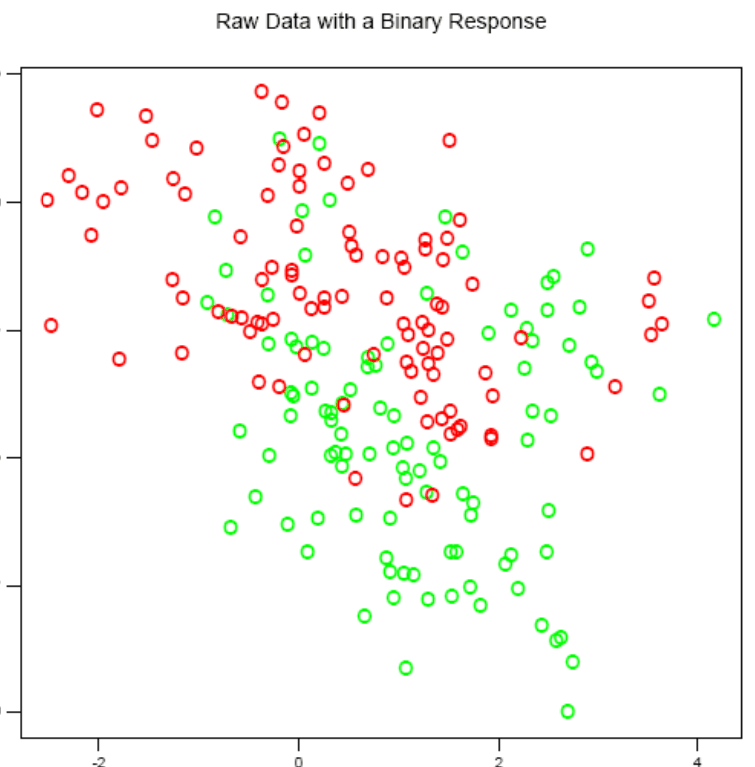
\includegraphics[width=0.43\linewidth,height=0.42\textheight,keepaspectratio]{images/05-lin_dataset.png}
\caption{The example problem (Hastie-Tibshirani-Friedman): 200 points of
two classes.}
\end{figure}

\subsection{Hyperplanes and decision
regions}\label{iperpiani-e-regioni-di-decisione}

The same models used for regression can be used for
\textbf{classification}, with categorical targets (\(0/1\) or
\(-1/+1\)). The expression \(\mathbf{w}^T\mathbf{x}\) defines a
\textbf{hyperplane}; we exploit the fact that
\(\mathbf{w}^T\mathbf{x}\) takes positive values on one side and
negative values on the other to decide which class a point belongs to.
The goal is to find, through learning, a \(\mathbf{w}\) that gives
good accuracy.

In two dimensions,
\(\mathbf{w}^T\mathbf{x} = w_0 + w_1 x_1 + w_2 x_2 = 0\) is a line:
the \textbf{decision boundary}.

\begin{figure}[htbp]
\centering
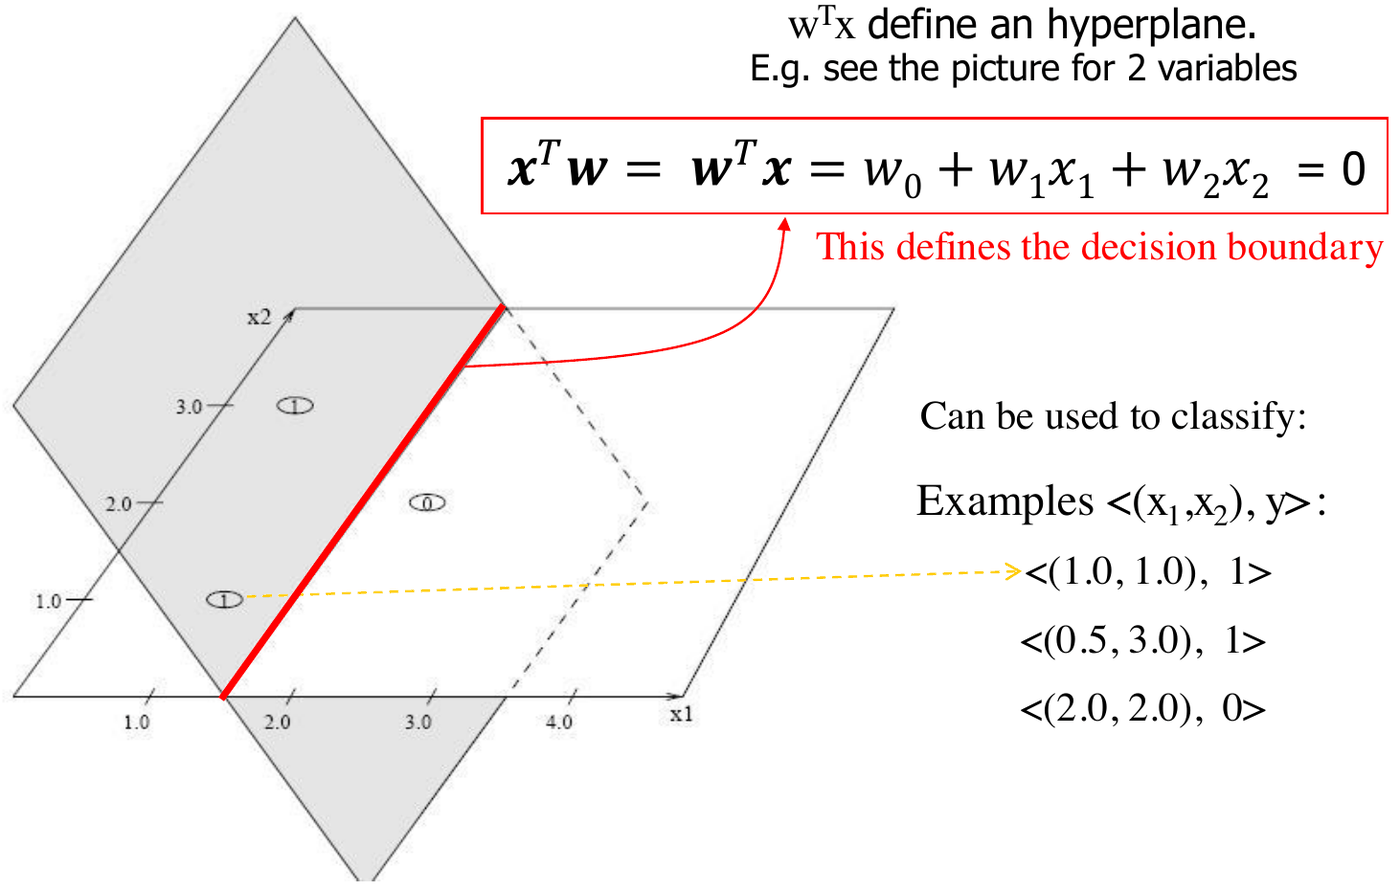
\includegraphics[width=0.71\linewidth,height=0.42\textheight,keepaspectratio]{images/05-lin_iperpiano.png}
\caption{The hyperplane \(\mathbf{w}^T\mathbf{x}\) and its intersection
with the input plane: the decision boundary.}
\end{figure}

To obtain a classifier a \textbf{threshold function} is applied: \[
h(\mathbf{x}) = \begin{cases} 1 & \text{if } \mathbf{w}^T\mathbf{x} + w_0 \ge 0 \\ 0 & \text{otherwise} \end{cases} \quad \text{(output in } [0,1]\text{)}, \qquad h(\mathbf{x}) = \operatorname{sign}(\mathbf{w}^T\mathbf{x} + w_0) \quad \text{(output in } [-1,+1]\text{)}.
\] Including \(w_0\) in \(\mathbf{w}\):
\(h(\mathbf{x}_p) = \operatorname{sign}(\mathbf{x}_p^T\mathbf{w}) = \operatorname{sign}\left(\sum_{i=0}^{n} x_{p,i} w_i\right)\).
This is the \textbf{Linear Threshold Unit} (LTU).

\begin{boxnote}{The bias as a threshold}

Saying \(\mathbf{w}^T\mathbf{x} + w_0 \ge 0\) is equivalent to saying
\(\mathbf{w}^T\mathbf{x} \ge -w_0\). The two forms identify the same
positive region, but the second highlights the role of the bias:
\(-w_0\) is the \textbf{threshold value} that the weighted combination
of the inputs must exceed to ``fire'' the \(+1\) output.

\end{boxnote}

\subsection{Using the model: two
examples}\label{usare-il-modello-due-esempi}

\begin{boxexample}{Earthquakes or nuclear explosions? (AIMA)}

Seismic data (1982--1990, Asia): \(x_1\) is the body wave magnitude,
\(x_2\) the surface wave magnitude. A learning algorithm finds the
boundary \(-4.9 + 1.7x_1 - x_2 = 0\). To classify a new event
\((6, 3)\): \[
h(6,3) = \operatorname{sign}(-4.9 + 1.7 \cdot 6 - 1 \cdot 3) = \operatorname{sign}(2.3) = +1 \;\Rightarrow\; \text{nuclear explosion.}
\] (Obtaining new training examples, in this case, is decidedly
expensive.)

\end{boxexample}

\begin{figure}[htbp]
\centering
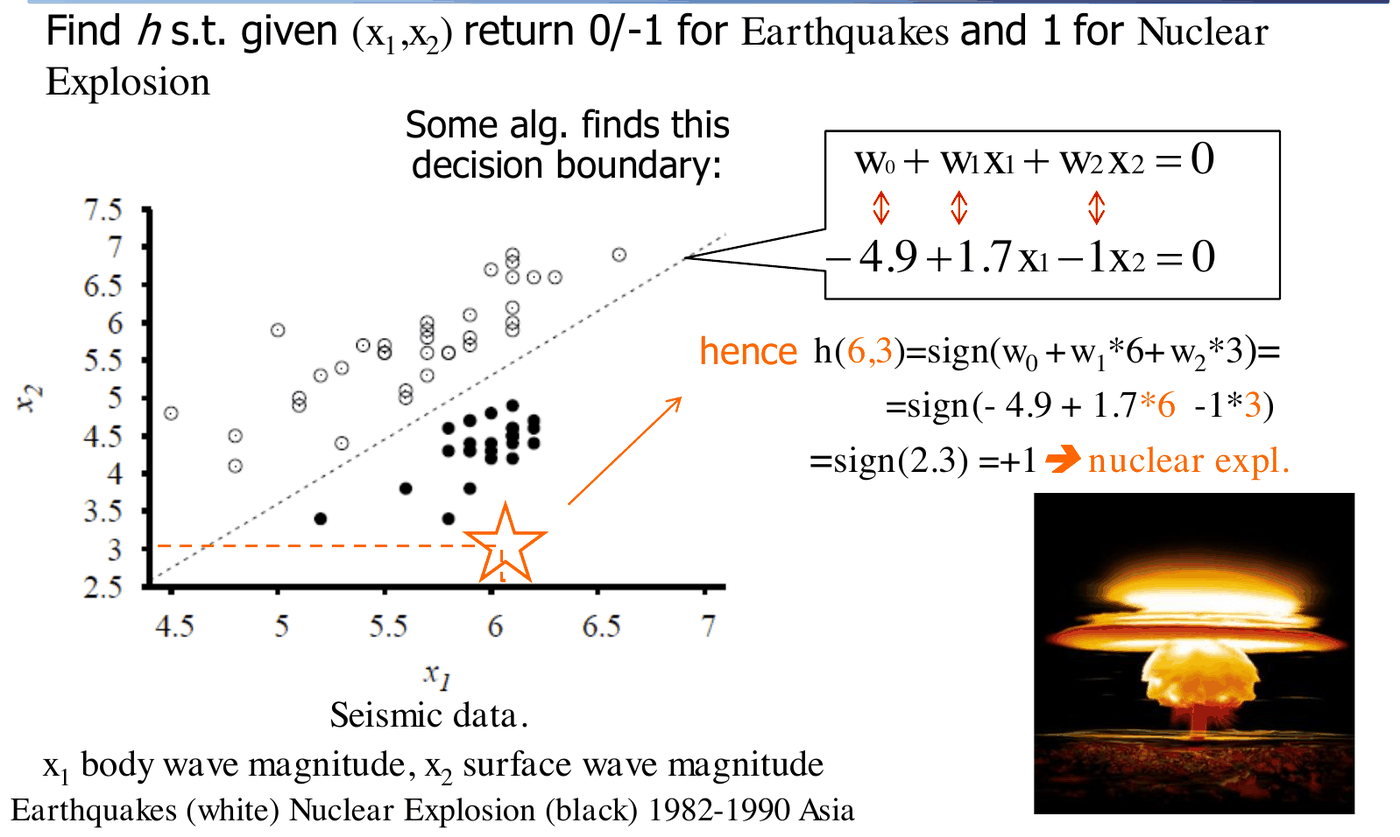
\includegraphics[width=0.80\linewidth,height=0.42\textheight,keepaspectratio]{images/05-lin_aima-sismi.png}
\caption{Classification of seismic data with a linear decision boundary.}
\end{figure}

\begin{boxexample}{Spam filter}

We want \(h(\text{mail}) = +1\) for spam and \(-1\) otherwise. The
features \(\phi_k(\text{mail})\) are for example the presence
(\(0/1\)) of words or phrases (``free money'') or the length
(integer): this is the \emph{bag of words} representation. Each weight
\(w_k\) expresses the contribution of the feature to the prediction:
positive for ``free money'', negative for ``.edu'' or ``unipi''. The
classification is
\(h_\mathbf{w}(\mathbf{x}) = \operatorname{sign}\left(\sum_k w_k \phi_k(\mathbf{x})\right)\):
if the weighted combination is positive, it is spam.

\end{boxexample}

\subsection{Useful properties of the
hyperplane}\label{proprietuxe0-utili-delliperpiano}

\begin{figure}[htbp]
\centering
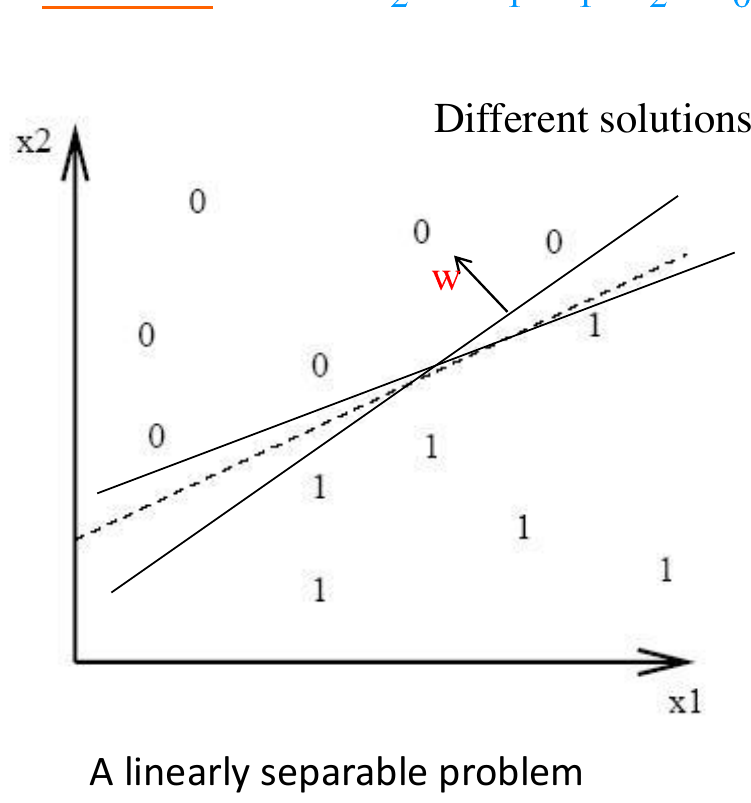
\includegraphics[width=0.43\linewidth,height=0.42\textheight,keepaspectratio]{images/05-lin_proprieta.png}
\caption{A linearly separable problem admits many separating
hyperplanes; \(\mathbf{w}\) is orthogonal to the hyperplane.}
\end{figure}

\begin{itemize}
\tightlist
\item
  If \(w_0 = 0\) the line passes through the \textbf{origin}.
\item
  If \(n > 2\) the boundary is a \textbf{hyperplane}.
\item
  \textbf{Scale freedom}: multiplying \(\mathbf{w}\) by a constant
  \(K\) does not change the boundary.
\item
  \textbf{\(\mathbf{w}\) is orthogonal to the hyperplane}: taking two
  points \(\mathbf{x}_a, \mathbf{x}_b\) on the hyperplane,
  \(\mathbf{w}^T\mathbf{x}_a + w_0 = 0\) and
  \(\mathbf{w}^T\mathbf{x}_b + w_0 = 0\); subtracting gives
  \(\mathbf{w}^T(\mathbf{x}_a - \mathbf{x}_b) = 0\), i.e.\
  \(\mathbf{w}\) is orthogonal to every vector lying on the
  hyperplane.
\item
  If a separating hyperplane exists, \textbf{many exist}, and hence
  also many algorithms to find them.
\end{itemize}

The equation of the line can be rewritten as
\(x_2 = -x_1 \frac{w_1}{w_2} - \frac{w_0}{w_2}\): trying to draw it
with different values of \(\mathbf{w}\) is a good exercise.

\section{The learning
problem}\label{il-problema-di-apprendimento}

\subsection{Formulation}\label{formulazione}

Given \(l\) examples \((\mathbf{x}_p, y_p)\) with \(y_p \in \{0,1\}\)
or \(\{-1,+1\}\) and a loss \(L\), we look for \(\mathbf{w}\)
minimising the empirical risk \[
R_{emp} = \frac{1}{l}\sum_{p=1}^{l} L\big(h(\mathbf{x}_p), y_p\big).
\] For classification, directly using the 0/1 loss on
\(\operatorname{sign}(\mathbf{w}^T\mathbf{x})\) makes the problem
hard: the function is \textbf{piecewise constant}, so the gradient is
zero almost everywhere and gives no indication of how to move, and one
ends up with combinatorial problems.

\subsection{Replacing the loss with a smooth
function}\label{sostituire-la-loss-con-una-funzione-liscia}

The idea is to replace the 0/1 loss with a \textbf{smooth and
differentiable} function, such as the squared error, applied directly
to the linear output \(\mathbf{w}^T\mathbf{x}\) (not to
\(h(\mathbf{x})\), which contains the sign): \[
E(\mathbf{w}) = \sum_{p=1}^{l}(y_p - \mathbf{x}_p^T\mathbf{w})^2 = \|\mathbf{y} - X\mathbf{w}\|^2.
\]

\begin{figure}[htbp]
\centering
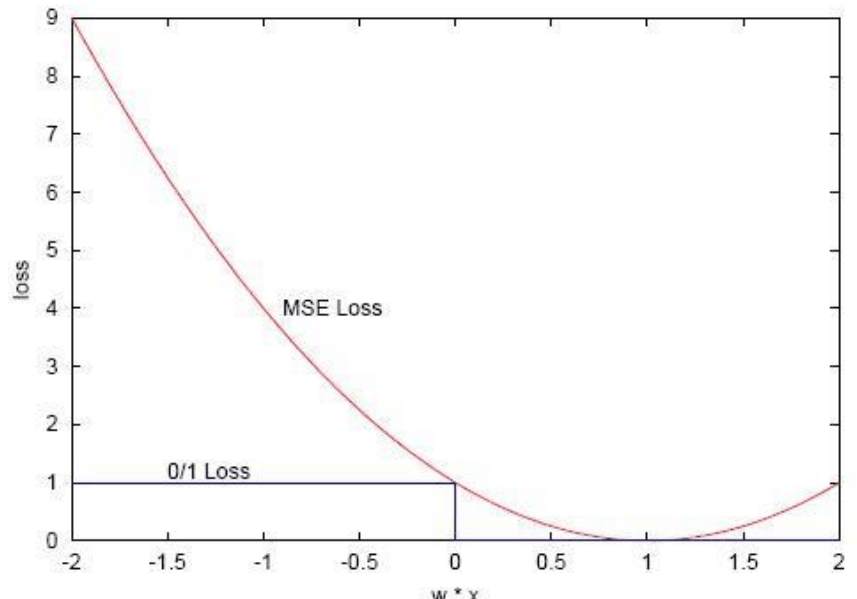
\includegraphics[width=0.54\linewidth,height=0.42\textheight,keepaspectratio]{images/05-lin_loss-smooth.png}
\caption{0/1 loss and squared loss for a pattern with target \(y = 1\):
both are minimised in the region \(\mathbf{w}^T\mathbf{x} > 0\).}
\end{figure}

Why does it work? With target \(y_p = 1\), minimising
\((1 - \mathbf{x}_p^T\mathbf{w})^2\) pushes
\(\mathbf{x}_p^T\mathbf{w}\) towards \(1\), hence positive: no
classification error. With \(y_p = -1\) it pushes it towards \(-1\).
Both losses are minimised in the same region (on the right in the
plot). The function is \textbf{quadratic}, so a minimum always exists
(but it is not necessarily unique). The same approach applies
identically to regression.

We now see two learning algorithms, both based on LMS and valid for
both regression and classification:

\begin{enumerate}
\def\labelenumi{\arabic{enumi}.}
\tightlist
\item
  a \textbf{direct approach} based on the \textbf{normal equations};
\item
  an \textbf{iterative approach} based on \textbf{gradient descent}.
\end{enumerate}

\subsection{Direct approach: the normal
equations}\label{approccio-diretto-le-equazioni-normali}

Differentiating \(E(\mathbf{w})\) with respect to the component
\(w_j\): \[
\frac{\partial E(\mathbf{w})}{\partial w_j} = \sum_{p=1}^{l} 2(y_p - \mathbf{x}_p^T\mathbf{w}) \frac{\partial (y_p - \mathbf{x}_p^T\mathbf{w})}{\partial w_j}.
\] In the dot product
\(\mathbf{x}_p^T\mathbf{w} = x_{p,1}w_1 + x_{p,2}w_2 + \dots\) the only
term that depends on \(w_j\) is \(x_{p,j}w_j\), whose derivative is
\(x_{p,j}\). Therefore: \[
\frac{\partial E(\mathbf{w})}{\partial w_j} = -2\sum_{p=1}^{l} (y_p - \mathbf{x}_p^T\mathbf{w})\, x_{p,j} = -2\sum_{p=1}^{l} \delta_p\, x_{p,j},
\] where \(\delta_p = y_p - \mathbf{x}_p^T\mathbf{w}\) is the error on
pattern \(p\). This form will come back in neural networks.

Setting the gradient to zero and switching to matrix notation we obtain
the \textbf{normal equations}: \[
(X^T X)\,\mathbf{w} = X^T \mathbf{y}.
\]

\begin{boxtheorem}{Least squares solution}

If \(X^TX\) is non-singular, the solution is unique: \[
\mathbf{w} = (X^TX)^{-1}X^T\mathbf{y} = X^+\mathbf{y},
\] where \(X^+\) is the \textbf{Moore-Penrose pseudoinverse} (defined
even if \(X\) is not invertible). Otherwise there are infinitely many
solutions, and the one with \textbf{minimum norm} of \(\mathbf{w}\) can
be chosen.

\end{boxtheorem}

In practice the \textbf{singular value decomposition} (SVD) is used:
\(X = U\Sigma V^T\) implies \(X^+ = V\Sigma^+U^T\), where \(\Sigma^+\)
is obtained by replacing each non-zero diagonal element with its
reciprocal. Applying the SVD one computes directly
\(\mathbf{w} = X^+\mathbf{y}\), obtaining the minimum-norm solution.
\textbf{This is the learning algorithm} of the direct approach; it is
implemented in all numerical libraries (Numerical Recipes, Armadillo,
NumPy, R, Matlab\ldots), with many variants for efficiency and
stability.

\subsection{Iterative approach: gradient
descent}\label{approccio-iterativo-la-discesa-del-gradiente}

Why look for other approaches if the direct solution exists? An
iterative approach makes it possible to obtain:

\begin{itemize}
\tightlist
\item
  \textbf{more efficient} solutions (the direct one is cubic in the
  size of the matrix);
\item
  \textbf{regularisation} (to reduce model complexity);
\item
  better approximation with noisy data, by stopping the search
  \textbf{before the minimum};
\item
  above all, a method that also applies to \textbf{non-linear
  models}. It is the basis of the fundamental approaches we will see
  (neural networks).
\end{itemize}

\subsubsection{The idea}\label{lidea}

The gradient
\(\frac{\partial E}{\partial w_j} = -2\sum_p (y_p - \mathbf{x}_p^T\mathbf{w})\, x_{p,j}\)
indicates the direction of \textbf{ascent} of the error. Moving in the
opposite direction (\(\Delta\mathbf{w} = -\nabla E(\mathbf{w})\)) we go
down towards the minimum. It is a \textbf{local search}: we start from
an initial weight vector and iteratively modify it to decrease the
error (\emph{steepest descent}).

\begin{figure}[htbp]
\centering
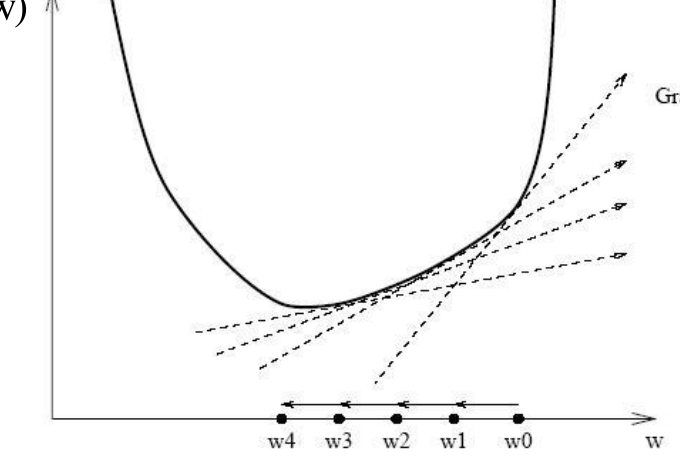
\includegraphics[width=0.46\linewidth,height=0.42\textheight,keepaspectratio]{images/05-lin_discesa-1d.png}
\caption{Gradient descent in one dimension: at each step the weight moves
in the direction opposite to the slope.}
\end{figure}

With two weights, the error surface \(E([w_0, w_1]^T)\) is a
\textbf{paraboloid} (convex quadratic function), and the negative
gradient is our ``compass'' to find the minimum.

\begin{figure}[htbp]
\centering
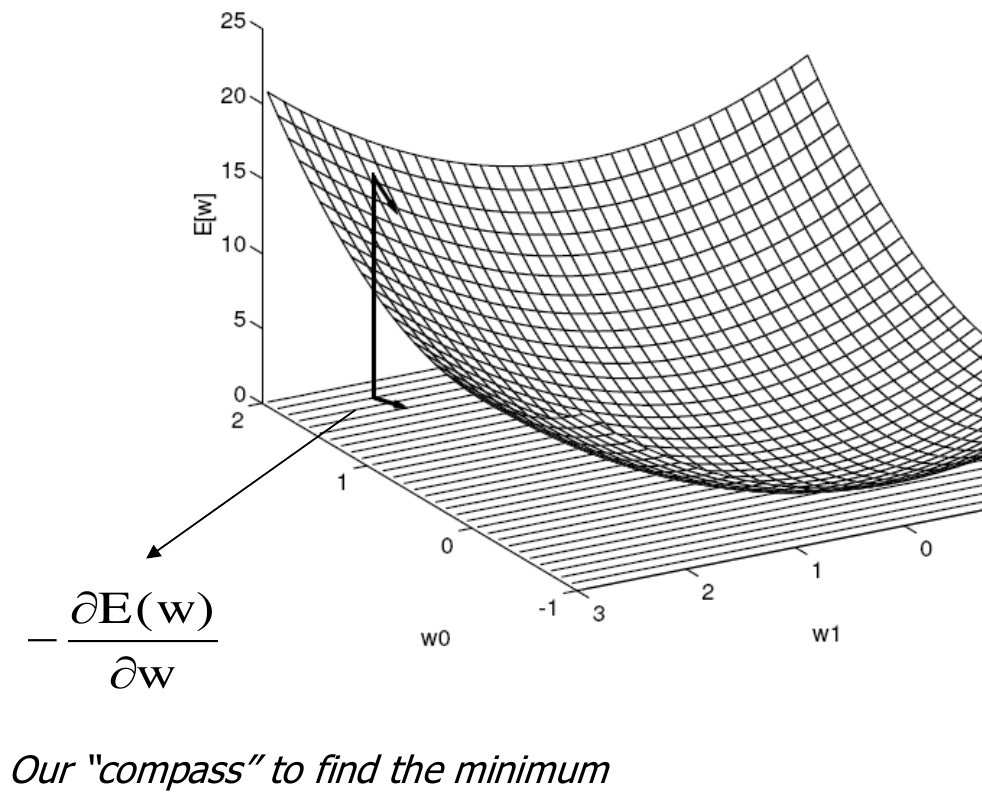
\includegraphics[width=0.54\linewidth,height=0.42\textheight,keepaspectratio]{images/05-lin_superficie-errore.png}
\caption{The error surface of a linear model with two weights: each
point of the \((w_0, w_1)\) plane is a hypothesis.}
\end{figure}

In general the vector \(\Delta\mathbf{w}\) has one component for each
weight: \[
\Delta\mathbf{w} = -\frac{\partial E(\mathbf{w})}{\partial \mathbf{w}} = \left( -\frac{\partial E}{\partial w_0}, -\frac{\partial E}{\partial w_1}, \dots, -\frac{\partial E}{\partial w_n} \right)^T,
\] and we can work in multidimensional spaces without needing to
visualise them.

\subsubsection{The learning rule (delta
rule)}\label{la-regola-di-apprendimento-delta-rule}

We move iteratively with a \textbf{learning rule}: \[
\mathbf{w}_{new} = \mathbf{w} + \eta\, \Delta\mathbf{w},
\] where \(\eta\) (eta) is the \textbf{learning rate} (\emph{step
size}), which controls the speed of descent.

\begin{boxabstract}{Gradient descent algorithm}

\begin{enumerate}
\def\labelenumi{\arabic{enumi}.}
\tightlist
\item
  Initialise \(\mathbf{w}\) with small values; fix \(0 < \eta < 1\).
\item
  Compute
  \(\Delta\mathbf{w} = -\frac{\partial E(\mathbf{w})}{\partial \mathbf{w}}\).
\item
  Update \(\mathbf{w}_{new} = \mathbf{w} + \eta\,\Delta\mathbf{w}\).
\item
  Repeat from step 2 until convergence or until \(E(\mathbf{w})\) is
  ``small enough''.
\end{enumerate}

\end{boxabstract}

Notes:

\begin{itemize}
\tightlist
\item
  using \(\Delta\mathbf{w}/l\) corresponds to \emph{least mean squares}
  (dividing by \(l\) will be the standard case);
\item
  \(\eta\) controls a \textbf{speed/stability} trade-off; it can be
  gradually reduced towards zero to guarantee convergence while
  avoiding oscillations around the minimum (many variants will be seen
  later).
\end{itemize}

\subsubsection{Batch and on-line}\label{batch-e-on-line}

\begin{itemize}
\tightlist
\item
  \textbf{Batch version}: the gradient is the sum over \textbf{all}
  \(l\) patterns, and the weights are updated after seeing the whole
  training set (an \textbf{epoch}). The gradient estimate is more
  ``precise''.
\item
  \textbf{On-line} (or \textbf{stochastic}, SGD) \textbf{version}: the
  weights are updated after \textbf{each} pattern, with the gradient
  of the single pattern: \[
  \frac{\partial E_p(\mathbf{w})}{\partial w_j} = -2(y_p - \mathbf{x}_p^T\mathbf{w})\, x_{p,j} = -\Delta_p w_j.
  \] The output of the second pattern is thus computed with weights
  already updated by the first, and so on. It makes progress at every
  example and can be faster, but it requires a smaller \(\eta\).
\end{itemize}

There are intermediate cases (\textbf{mini-batch}), which we will see
later.

\begin{figure}[htbp]
\centering
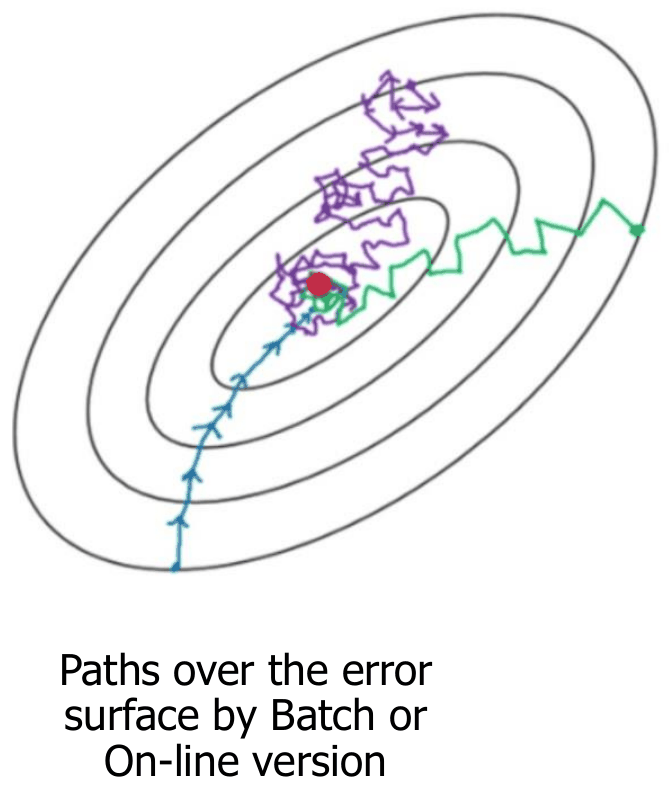
\includegraphics[width=0.40\linewidth,height=0.42\textheight,keepaspectratio]{images/05-lin_batch-online.png}
\caption{Paths on the error surface: batch (blue, smooth) and on-line
(purple and green, more irregular).}
\end{figure}

\begin{figure}[htbp]
\centering
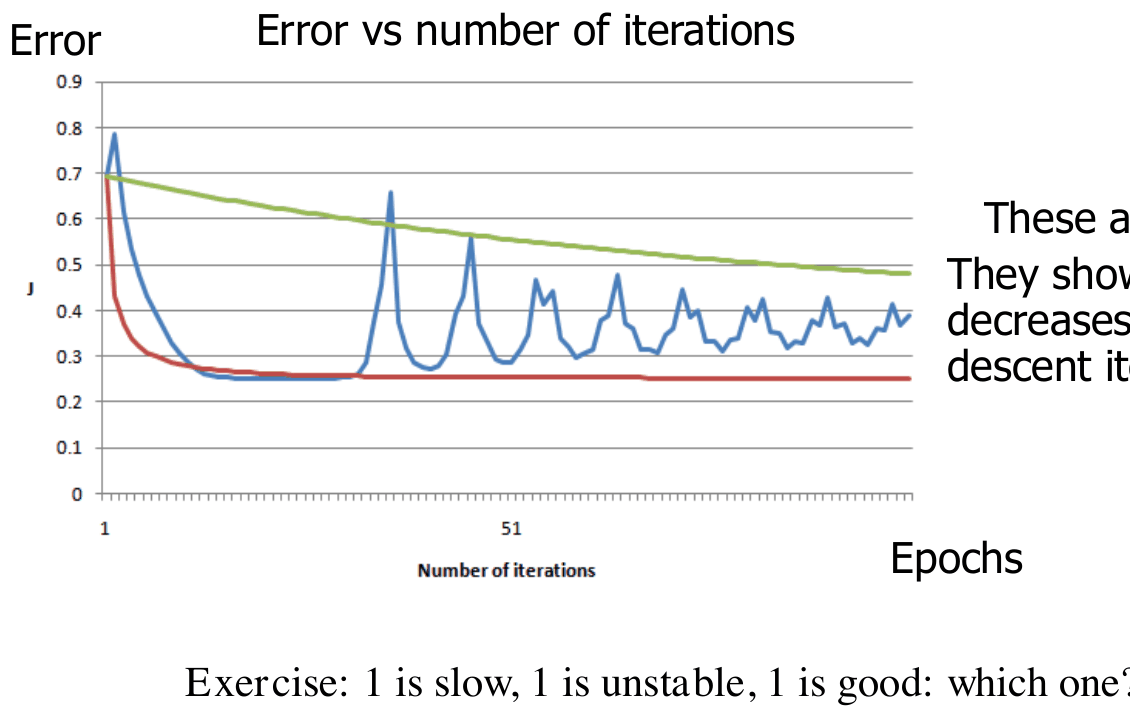
\includegraphics[width=0.63\linewidth,height=0.42\textheight,keepaspectratio]{images/05-lin_curve-apprendimento.png}
\caption{Learning curves: the error as a function of the iterations
(epochs).}
\end{figure}

\begin{boxquestion}{Exercise: which curve is slow, which unstable, which good?}

The \textbf{green} curve decreases very slowly (learning rate too
small); the \textbf{blue} one shows spikes and oscillations (learning
rate too large, unstable); the \textbf{red} one decreases quickly and
stabilises (good).

\end{boxquestion}

\subsubsection{Interpretation: an error-correction
rule}\label{interpretazione-una-regola-di-correzione-dellerrore}

Summing up, \[
\Delta w_j = 2\sum_{p=1}^{l} \underbrace{(y_p - \mathbf{x}_p^T\mathbf{w})}_{\delta_p}\, x_{p,j}, \qquad \mathbf{w}_{new} = \mathbf{w} + \eta\,\Delta\mathbf{w}
\] (the constant 2 can be omitted, absorbing it into \(\eta\)). It is
an \textbf{error-correction} rule, called the \textbf{Widrow-Hoff
rule} or \textbf{delta rule}: each \(w_j\) changes \textbf{in
proportion to the error} (target − output).

\begin{itemize}
\tightlist
\item
  If the error is 0, there is no correction.
\item
  With input \(x_j > 0\): if the error is positive (output too low),
  positive delta → \(w_j\) increases → the output increases → the error
  decreases.
\item
  With input \(x_j > 0\): if the error is negative (output too high),
  negative delta → \(w_j\) decreases → the output decreases → the error
  decreases.
\item
  With a negative input the signs are reversed, with a zero input the
  weight does not change: the input ``decides'' how much and in which
  direction each weight is responsible for the error.
\end{itemize}

We learn from previous mistakes: \emph{``by trying and failing one
learns''} (Goethe).

\begin{figure}[htbp]
\centering
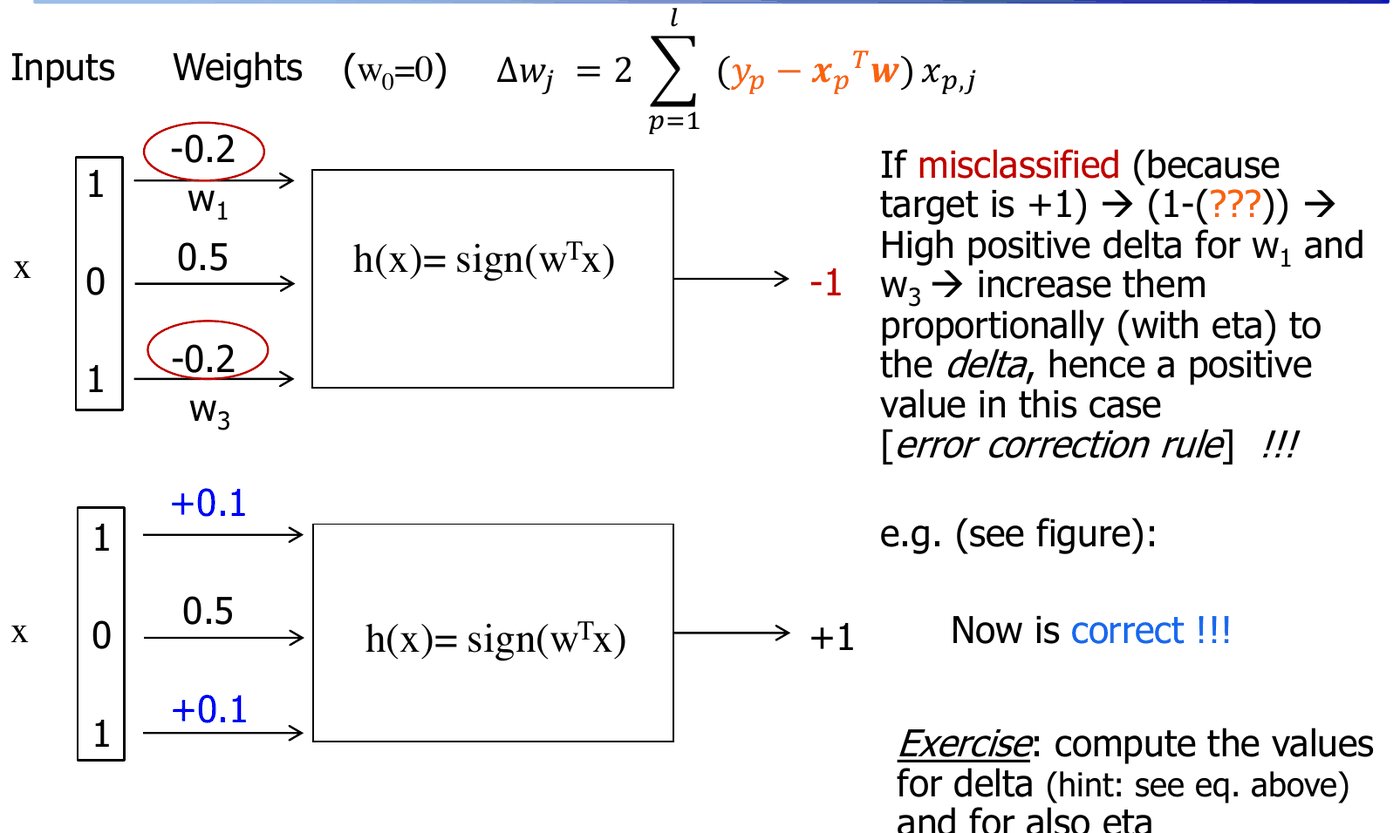
\includegraphics[width=0.86\linewidth,height=0.42\textheight,keepaspectratio]{images/05-lin_delta-rule.png}
\caption{The delta rule at work: the weights of the active inputs are
increased until the pattern is correctly classified.}
\end{figure}

In the example, the input is \((1, 0, 1)\) with weights
\((-0.2;\ 0.5;\ -0.2)\) and \(w_0 = 0\):
\(\mathbf{w}^T\mathbf{x} = -0.4\), so the output is \(-1\) but the
target is \(+1\). The delta is positive: \(w_1\) and \(w_3\) (whose
inputs are 1) are increased, while \(w_2\) (input 0) stays unchanged.
After the correction (\(w_1 = w_3 = +0.1\)) we have
\(\mathbf{w}^T\mathbf{x} = 0.2 > 0\) and the output is correct.

\begin{boxtip}{Why gradient descent is so important}

It is a simple and effective local search method that makes it
possible to explore an \textbf{infinite and continuous} hypothesis
space. It always applies when \(H\) is continuous and the loss is
differentiable, \textbf{not only to linear models}: it will be the
basis for training neural networks and deep learning. There are many
improvements (Newton and quasi-Newton methods, conjugate
gradient\ldots).

\end{boxtip}

\subsection{Summary for
classification}\label{riepilogo-per-la-classificazione}

\begin{itemize}
\tightlist
\item
  The model is trained on TR with LMS applied to
  \(\mathbf{w}^T\mathbf{x}\), through the same gradient descent used
  for regression.
\item
  The model is \textbf{used} to classify by applying the threshold:
  \(h(\mathbf{x}) = \operatorname{sign}(\mathbf{w}^T\mathbf{x})\).
\item
  The error can be evaluated as \textbf{classification error} (0/1
  loss, number of wrong patterns), not only as MSE: \[
  \text{mean\_err} = \frac{1}{l}\sum_{p=1}^{l} L\big(h(\mathbf{x}_p), d_p\big) = \frac{\text{num\_err}}{l}, \qquad \text{accuracy} = \frac{l - \text{num\_err}}{l}.
  \]
\end{itemize}

\subsection{Back to the problem: is it a good
solution?}\label{torniamo-al-problema-uxe8-una-buona-soluzione}

\begin{figure}[htbp]
\centering
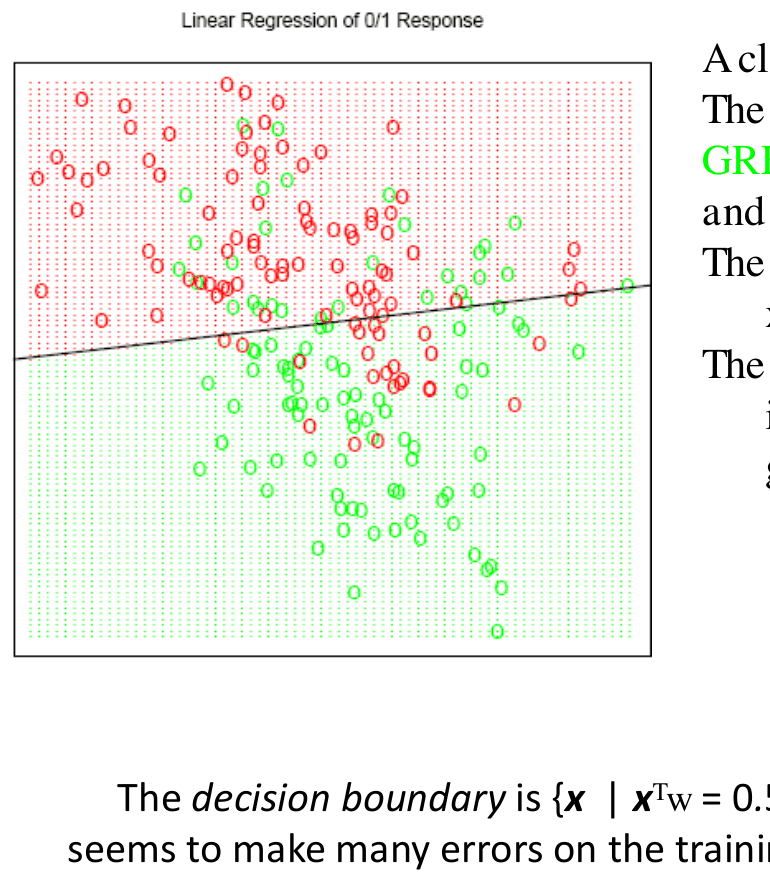
\includegraphics[width=0.46\linewidth,height=0.42\textheight,keepaspectratio]{images/05-lin_htf-lineare.png}
\caption{Linear solution to the example problem: classes encoded as GREEN
= 0, RED = 1, boundary \(\mathbf{x}^T\mathbf{w} = 0.5\).}
\end{figure}

The boundary \(\{\mathbf{x} \mid \mathbf{x}^T\mathbf{w} = 0.5\}\) is
linear and seems to make many errors on the training set. Is it a bad
solution? It depends on how the data were generated:

\begin{itemize}
\tightlist
\item
  \textbf{Scenario 1}: each class is generated by a Gaussian with
  uncorrelated components, same variance and different means. In this
  case the linear rule is \textbf{almost optimal}: the overlap between
  the classes is unavoidable (due to noise in the data).
\item
  \textbf{Scenario 2}: each class is a mixture of 10 Gaussians. In this
  case the linear model is \textbf{too rigid}, and the next models are
  needed.
\end{itemize}

\begin{boxnote}{Least squares and maximum likelihood}

Least squares corresponds to the \textbf{maximum likelihood} criterion
if the experimental errors are normally distributed.

\end{boxnote}

\subsection{Inductive bias of the linear
model}\label{bias-induttivo-del-modello-lineare}

\begin{itemize}
\tightlist
\item
  \textbf{Language bias}: \(H\) is the set of linear functions, which
  can be very restrictive and rigid.
\item
  \textbf{Search bias}: ordered search guided by least squares
  minimisation. One might prefer a different method, which for example
  restricts the parameter values, obtaining solutions with different
  properties (in particular with respect to generalisation).
\end{itemize}

Even for a ``simple'' model there are many possibilities: a
principled approach (ML theory) is needed.

\section{Limits of linear models}\label{limiti-dei-modelli-lineari}

\subsection{Regression of non-linear
problems}\label{regressione-di-problemi-non-lineari}

If the target function is not linear (like the sine of the polynomial
example), a line is \textbf{too poor} a solution: it is the \(M = 1\)
case already seen, well within the underfitting zone.

\subsection{Classification: linear
separability}\label{classificazione-separabilituxe0-lineare}

\begin{boxdefinition}{Linear separability}

Two sets of points in the plane are \textbf{linearly separable} if they
can be completely separated by a single line. In general, two groups
are linearly separable in an \(n\)-dimensional space if they can be
separated by a hyperplane of dimension \(n-1\).

\end{boxdefinition}

The linear decision boundary provides exact solutions \textbf{only}
for linearly separable sets.

The linear model can represent, for example,
\textbf{conjunctions}. The conjunction \(x_1 \wedge x_2 \wedge x_4\) is
realised with
\(1 \cdot x_1 + 1 \cdot x_2 + 0 \cdot x_3 + 1 \cdot x_4 \ge 2.5\)
(true only if all three are 1); the two-variable AND with
\(x_1 + x_2 \ge 1.5\). The weights \(\mathbf{w}\) of these solutions
can be learned.

\begin{figure}[htbp]
\centering
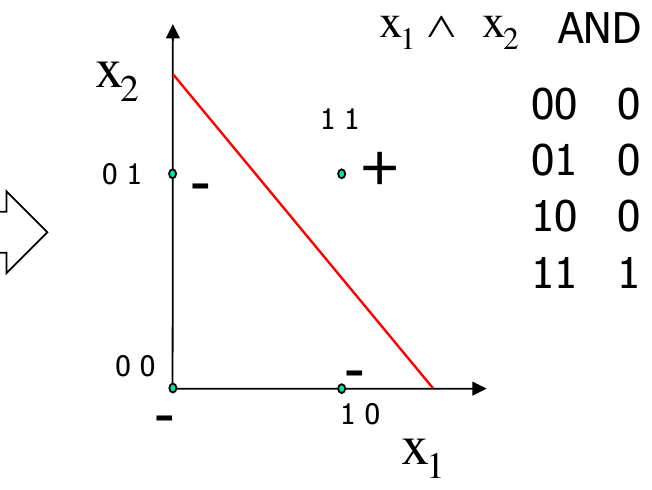
\includegraphics[width=0.40\linewidth,height=0.42\textheight,keepaspectratio]{images/05-lin_and.png}
\caption{AND is linearly separable.}
\end{figure}

But not everything is separable:

\begin{itemize}
\tightlist
\item
  \textbf{3 points}: can we always find a hyperplane for every
  assignment of labels? Yes, \textbf{if they are not collinear}. If
  they are collinear, the labelling ``1--0--1'' (0 in the middle) is
  not separable.
\item
  \textbf{4 points}: no. There is a labelling for which no linear
  classifier is perfect: \textbf{XOR} (\(00 \mapsto 0\),
  \(01 \mapsto 1\), \(10 \mapsto 1\), \(11 \mapsto 0\)), in which the
  positives lie on one diagonal and the negatives on the other.
\end{itemize}

\begin{figure}[htbp]
\centering
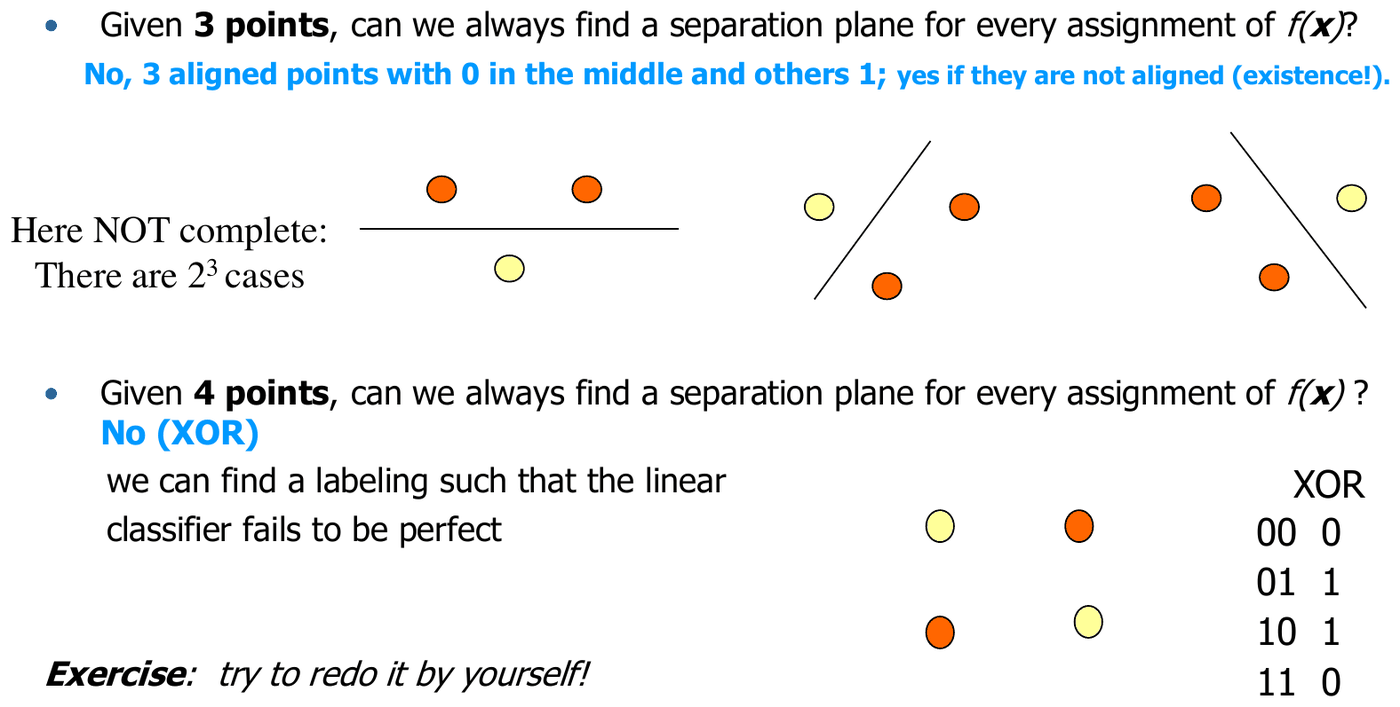
\includegraphics[width=0.86\linewidth,height=0.42\textheight,keepaspectratio]{images/05-lin_xor.png}
\caption{Limits of linear separation: three non-collinear points are
always separable, XOR on four points is not.}
\end{figure}

\begin{boxnote}{Preview}

This ``counting how many labellings can be separated'' is exactly the
idea of the \textbf{VC-dimension}: a hyperplane in the plane separates
all labellings of 3 (non-collinear) points, but not of 4. The
VC-dimension of lines in the plane is therefore 3.

\end{boxnote}

\section{Extending the linear
model}\label{estendere-il-modello-lineare}

\subsection{``Linear'' in the parameters, not in the
inputs}\label{lineare-nei-parametri-non-negli-input}

In parametric statistical models, \textbf{``linear'' does not refer to
the line}, but to the way the \textbf{coefficients \(\mathbf{w}\)}
appear in the equation. Transformed inputs such as
\(x, x^2, x^3, \dots\) can therefore be used to model non-linear
relationships between input and output, keeping \textbf{the same
learning machinery} (least squares). This is exactly the polynomial
regression of the introduction: \[
h_\mathbf{w}(x) = w_0 + w_1 x + w_2 x^2 + \dots + w_M x^M = \sum_{j=0}^{M} w_j x^j.
\]

\subsection{Linear Basis Expansion
(LBE)}\label{linear-basis-expansion-lbe}

\begin{boxdefinition}{Linear basis expansion}

\[
h_\mathbf{w}(\mathbf{x}) = \sum_{k=0}^{K} w_k\, \phi_k(\mathbf{x})
\] where the \(\phi_k: \mathbb{R}^n \to \mathbb{R}\) are fixed
transformations of the input. The input vector is augmented with new
variables derived from \(\mathbf{x}\).

\end{boxdefinition}

Examples of \(\phi\):

\begin{itemize}
\tightlist
\item
  \textbf{polynomial} representation: \(\phi(\mathbf{x}) = x_j^2\),
  \(\phi(\mathbf{x}) = x_j x_i\), \ldots;
\item
  non-linear transformations of single inputs: \(\log(x_j)\),
  \(\sqrt{x_j}\), \ldots;
\item
  transformations of multiple inputs:
  \(\phi(\mathbf{x}) = \|\mathbf{x}\|\);
\item
  splines, \ldots{}
\end{itemize}

For example:
\(h(\mathbf{x}) = w_1x_1 + w_2x_2 + w_3\log(x_2) + w_4\log(x_3) + w_5(x_2x_3) + w_0\).

Typically the number of parameters becomes \(K > n\). The model is
\textbf{linear in the parameters} (and in the \(\phi\)), not in
\(\mathbf{x}\): the same learning algorithm is used. This holds for
regression and also for classification (it is enough to apply the
threshold to \(\sum_k w_k\phi_k(\mathbf{x})\)).

\begin{boxwarning}{Pros and cons of basis expansion}

\textbf{Pros}: it models more complex relationships, it is more
expressive.

\textbf{Cons}: - with many basis functions one easily risks
\textbf{overfitting}, so complexity control methods are needed
(complexity meant as flexibility, i.e.\ VC-dim, not as computational
cost); - the \textbf{curse of dimensionality}: the volume of the space
grows so fast that the available data become sparse and are no longer
enough to support the complexity of the model; - the \(\phi\) are
\textbf{fixed before} seeing the data. The alternative is adaptive
models, non-linear in the parameters, such as \textbf{neural networks}
(which learn the \(\phi\)) and \textbf{SVMs}.

The question then remains open: which \(\phi\) should be chosen?
(``dictionary'' approaches).

\end{boxwarning}

\section{Regularisation: complexity
control}\label{regolarizzazione-il-controllo-della-complessituxe0}

How can model complexity be controlled? Among the many approaches there
is \textbf{coefficient shrinkage}.

\subsection{Ridge regression (Tikhonov
regularisation)}\label{ridge-regression-regolarizzazione-di-tikhonov}

A term that \textbf{penalises large weights} is added to the loss: \[
\text{Loss}(\mathbf{w}) = \underbrace{\sum_{p=1}^{l}(y_p - \mathbf{x}_p^T\mathbf{w})^2}_{\text{error term (} R_{emp}\text{)}} + \underbrace{\lambda\,\|\mathbf{w}\|^2}_{\text{penalty term}}, \qquad \|\mathbf{w}\|^2 = \sum_j w_j^2.
\] \(\lambda\) is the \textbf{regularisation hyperparameter}, a small
positive value chosen during \textbf{model selection}. The resulting
model is \emph{smoother}: models with small or zero weights are
favoured, i.e.\ models that use fewer terms, hence less complex.

\begin{boxnote}{Loss and Error are no longer synonyms}

From here on \textbf{Loss} denotes the objective function used for
training (error + penalty), while \textbf{Error} \(E\) denotes the
measure of the model's error (the data term). So far we had treated
them as equivalent.

\end{boxnote}

\begin{boxtip}{The learning goal changes}

With regularisation the goal is redefined: we no longer want
\textbf{only} the model that best fits the data, but \textbf{the
simplest model that fits the data well}. The loss is a balance between
two pans: - \textbf{fit to the data} (training error,
\(\sum_p(y_p - \mathbf{w}^T\mathbf{x}_p)^2\)): pushes the model to
follow the data and minimise the residuals; - \textbf{model
simplicity} (Tikhonov penalty, \(\|\mathbf{w}\|^2\)): punishes large
weights, making the model smoother, simpler and better able to
generalise;

and the \textbf{regularisation parameter} \(\lambda\) decides how much
weight to give to the penalty.

\end{boxtip}

\subsubsection{Solution}\label{soluzione}

\begin{itemize}
\tightlist
\item
  \textbf{Direct approach}:
  \(\mathbf{w} = (X^TX + \lambda I)^{-1}X^T\mathbf{y}\). The matrix
  \(X^TX + \lambda I\) is \textbf{always invertible} (for
  \(\lambda > 0\)): a numerical advantage too.
\item
  \textbf{Gradient approach}: we still follow the negative gradient of
  the loss. The derivative of the penalty term with respect to \(w_j\)
  is \(2\lambda w_j\), so the new rule is \[
  \mathbf{w}_{new} = \mathbf{w} + \eta\,\Delta\mathbf{w} - 2\lambda\mathbf{w},
  \] where \(\Delta\mathbf{w}\) is the negative gradient of the error
  term alone (multiplied by \(\eta\)), while the penalty is multiplied
  directly by \(\lambda\). This is the \textbf{weight decay} technique:
  even with zero error gradient, at each step every weight is reduced
  by a fraction of its value.
\end{itemize}

\subsubsection{\texorpdfstring{The trade-off governed by
\(\lambda\)}{The trade-off governed by \textbackslash lambda}}\label{il-compromesso-governato-da-lambda}

\begin{itemize}
\tightlist
\item
  \textbf{Small \(\lambda\)}: when minimising the loss the error term
  dominates; we obtain a model that is too complex (high-norm
  weights), with a risk of \textbf{overfitting}.
\item
  \textbf{Large \(\lambda\)}: the penalty dominates; the error on the
  data may grow too much, and we move towards \textbf{underfitting}.
\end{itemize}

The great advantage is that we have a \textbf{concrete realisation of
complexity control}, easy to implement and of general applicability.

\begin{boxtip}{Tikhonov and SLT}

The penalty pushes all weights towards small values (some even to
zero), achieving complexity control: we obtain a model with a lower (or
more suitable) VC-dimension, and the trade-off is controlled by
\textbf{a single parameter}, \(\lambda\). In the SLT bound plot,
increasing \(\lambda\) amounts to moving to the left (less
complexity): a well-chosen \(\lambda\) brings us close to the minimum
of the bound on \(R\).

\end{boxtip}

\subsubsection{Effect on the degree-9
polynomial}\label{effetto-sul-polinomio-di-grado-9}

Let us go back to the degree-9 polynomial with 10 points, which without
regularisation (\(\lambda = 0\)) had zero training error and very
strong overfitting.

\begin{figure}[htbp]
\centering
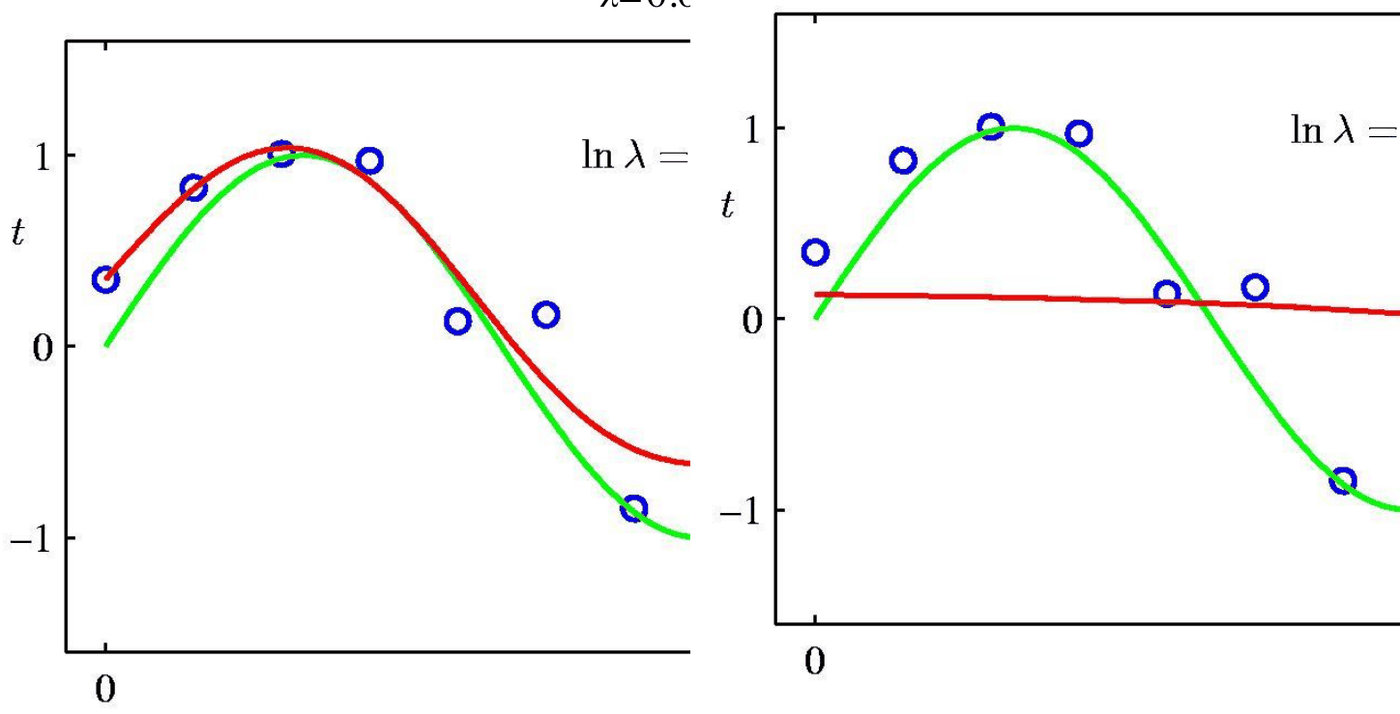
\includegraphics[width=0.80\linewidth,height=0.42\textheight,keepaspectratio]{images/05-lin_regolarizzazione.png}
\caption{Regularised degree-9 polynomial: with \(\ln\lambda = -18\)
(left) the curve is smooth and follows the true function well; with
\(\ln\lambda = 0\) (right) it is too flat.}
\end{figure}

With a suitable \(\lambda\) (\(\ln\lambda = -18\), i.e.\
\(\lambda \approx 1.5 \cdot 10^{-8}\)) the model works well: it is
\textbf{worse on the training set} but reduces overfitting. With
\(\lambda\) too high (\(\ln\lambda = 0\), i.e.\ \(\lambda = 1\)) we
end up in underfitting.

\begin{figure}[htbp]
\centering
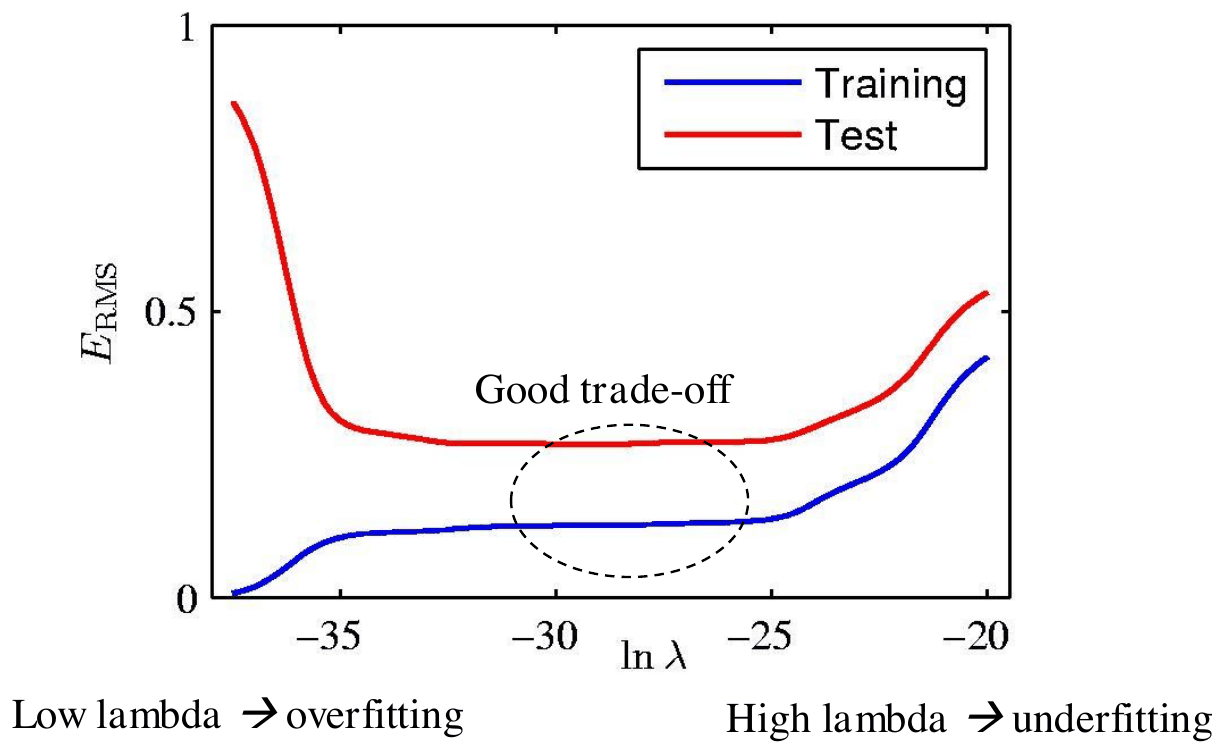
\includegraphics[width=0.63\linewidth,height=0.42\textheight,keepaspectratio]{images/05-lin_rms-lambda.png}
\caption{Training and test \(E_{RMS}\) as \(\ln\lambda\) varies:
overfitting on the left, underfitting on the right, the good trade-off
in the middle.}
\end{figure}

The coefficients also show the effect of regularisation:

{\def\LTcaptype{none} % do not increment counter
\begin{longtable}[]{@{}
  >{\raggedright\arraybackslash}p{(\linewidth - 6\tabcolsep) * \real{0.2500}}
  >{\raggedright\arraybackslash}p{(\linewidth - 6\tabcolsep) * \real{0.2500}}
  >{\raggedright\arraybackslash}p{(\linewidth - 6\tabcolsep) * \real{0.2500}}
  >{\raggedright\arraybackslash}p{(\linewidth - 6\tabcolsep) * \real{0.2500}}@{}}
\toprule\noalign{}
\begin{minipage}[b]{\linewidth}\raggedright
\end{minipage} & \begin{minipage}[b]{\linewidth}\raggedright
\(\ln\lambda = -\infty\) (\(\lambda = 0\))
\end{minipage} & \begin{minipage}[b]{\linewidth}\raggedright
\(\ln\lambda = -18\)
\end{minipage} & \begin{minipage}[b]{\linewidth}\raggedright
\(\ln\lambda = 0\)
\end{minipage} \\
\midrule\noalign{}
\endhead
\bottomrule\noalign{}
\endlastfoot
\(w_0^*\) & 0.35 & 0.35 & 0.13 \\
\(w_1^*\) & 232.37 & 4.74 & −0.05 \\
\(w_2^*\) & −5321.83 & −0.77 & −0.06 \\
\(w_3^*\) & 48568.31 & −31.97 & −0.05 \\
\(w_4^*\) & −231639.30 & −3.89 & −0.03 \\
\(w_5^*\) & 640042.26 & 55.28 & −0.02 \\
\(w_6^*\) & −1061800.52 & 41.32 & −0.01 \\
\(w_7^*\) & 1042400.18 & −45.95 & −0.00 \\
\(w_8^*\) & −557682.99 & −91.53 & 0.00 \\
\(w_9^*\) & 125201.43 & 72.68 & 0.01 \\
\end{longtable}
}

The huge weights of the unregularised case are drastically reduced:
regularisation ``tames'' the oscillations.

\subsection{Other regularisation
techniques}\label{altre-tecniche-di-regolarizzazione}

\begin{itemize}
\tightlist
\item
  \textbf{Ridge regression} (\(\|\cdot\|_2\) norm): penalises the
  square of the weights and tends to make \textbf{all} weights
  smaller.
\item
  \textbf{Lasso} (\(\|\cdot\|_1\) norm): penalises the absolute value
  and tends to bring \textbf{some weights exactly to zero} (leaving
  others large) → a form of \textbf{feature selection}. Unfortunately
  the absolute value makes the loss non-differentiable (at zero), and
  other approaches are needed.
\item
  \textbf{Elastic net}: uses both norms.
\end{itemize}

\begin{boxtip}{Why does L1 zero out weights and L2 does not?}

The gradient of \(\lambda w^2\) is \(2\lambda w\): it becomes tiny when
\(w\) is close to zero, so the push towards zero fades and the weight
stays small but non-zero. The (sub-)gradient of \(\lambda|w|\) is
instead \(\lambda\operatorname{sign}(w)\): a \textbf{constant} push
towards zero, even for weights that are already small, which brings
them exactly to zero if the error term does not ``defend'' them.

\end{boxtip}

\subsection{Other improvements
(optional)}\label{altri-miglioramenti-opzionali}

\begin{itemize}
\tightlist
\item
  \textbf{Data augmentation}: adding noise to the inputs teaches the
  model to ignore irrelevant variations (robustness and
  regularisation); oversampling helps with unbalanced datasets.
\item
  \textbf{Derived inputs}: a small number of new variables are used,
  linear combinations of the inputs (Principal Component Regression,
  Partial Least Squares).
\end{itemize}

\subsection{Multi-class classification
(optional)}\label{classificazione-multi-classe-opzionale}

Two simple approaches:

\begin{itemize}
\tightlist
\item
  \textbf{1-of-K} encoding of the classes (e.g.\ red, green, blue →
  \((0,0,1), (0,1,0), (1,0,0)\)) and one linear model for each
  component;
\item
  \textbf{OVA} (\emph{one-vs-all}): \(K\) binary classifiers are
  trained, each distinguishing one class from all the others; to
  classify, the one with the highest (most positive) output is chosen;
\item
  \textbf{AVA} (\emph{all-vs-all}, \emph{one-vs-one}): one classifier
  for each pair of classes (\(K(K-1)/2\) distinct classifiers); the
  class with the maximum sum of outputs or with the most votes wins.
  Each classifier is trained on less data.
\end{itemize}

With many classes \textbf{masking} phenomena may occur (a class
``hidden'' by the others). There are more sophisticated approaches and
models with native multiple outputs. Other well-known linear
classifiers are \textbf{Linear Discriminant Analysis} and
\textbf{logistic regression} (which directly models
\(P(y \mid \mathbf{x})\)).

\subsection{A look ahead}\label{uno-sguardo-avanti}

\begin{itemize}
\tightlist
\item
  The \textbf{Perceptron} (Rosenblatt, 1958, biologically inspired)
  minimises only the misclassifications and is the basis of
  \textbf{neural networks}: several units organised in layers, which
  implement an \textbf{adaptive basis expansion} (the \(\phi\) are
  learned), i.e.\ \emph{representation learning}, trained with gradient
  descent.
\item
  \textbf{SVMs} (Vapnik, 1996) regularise through \textbf{margin
  maximisation} between the classes and enlarge the feature space with
  basis expansion (e.g.\ polynomials).
\end{itemize}

Both implement a flexible non-linear approximation for classification
and regression.

\begin{boxabstract}{Lessons learned from linear models}

\begin{itemize}
\tightlist
\item
  It is possible to \textbf{learn by tuning free parameters}
  \(\mathbf{w}\), searching in a continuous space guided by a loss
  function.
\item
  The problem is formulated as \textbf{LMS} and two algorithms are
  derived: \textbf{direct} (normal equations, SVD) and
  \textbf{iterative} (gradient descent, delta rule).
\item
  Linear models have a strong \textbf{language bias} (only linearly
  separable problems).
\item
  Two key concepts of the common thread of the course: \textbf{basis
  expansion} (more \textbf{flexibility}) and \textbf{regularisation}
  (\textbf{complexity control}). We will find them again, in different
  forms, in neural networks and SVMs.
\end{itemize}

\end{boxabstract}

\section{K-nearest neighbors}\label{k-nearest-neighbors}

Now we move to the opposite extreme: from a rigid approach to a
\textbf{very flexible} (and local) one.

\subsection{Eager and lazy
learning}\label{apprendimento-eager-e-lazy}

With respect to the \emph{timing} of learning we distinguish:

\begin{itemize}
\tightlist
\item
  \textbf{eager}: the training data are analysed and an
  \textbf{explicit hypothesis} is built (like the linear model);
\item
  \textbf{lazy}: the data are stored and we wait for a test point;
  only then is an ad hoc hypothesis built to classify that point.
\end{itemize}

\subsection{1-nearest neighbor}\label{nearest-neighbor}

\begin{boxdefinition}{1-NN algorithm}

\begin{enumerate}
\def\labelenumi{\arabic{enumi}.}
\tightlist
\item
  Store the training data \(\langle \mathbf{x}_p, y_p\rangle\),
  \(p = 1,\dots,l\).
\item
  Given an input \(\mathbf{x}\) (of dimension \(n\)), find the nearest
  training example: \[
  i(\mathbf{x}) = \arg\min_p d(\mathbf{x}, \mathbf{x}_p),
  \] for example with the Euclidean distance
  \(d(\mathbf{x}, \mathbf{x}_p) = \sqrt{\sum_{t=1}^{n}(x_t - x_{p,t})^2} = \|\mathbf{x} - \mathbf{x}_p\|\).
\item
  Return \(y_i\).
\end{enumerate}

\end{boxdefinition}

1-NN is \textbf{very flexible}: on the training set it makes
\textbf{zero errors} (each point is its own nearest neighbour). The
decision boundary is not linear and is very irregular, perhaps
needlessly noisy (for example in scenario 1, where we know that the
optimal solution is almost linear). And on the test data?

\subsection{K-nearest neighbors}\label{k-nearest-neighbors-1}

A natural way to classify a new point is to look at its
\textbf{neighbours} and take their average: \[
\text{avg}_k(\mathbf{x}) = \frac{1}{k}\sum_{\mathbf{x}_i \in N_k(\mathbf{x})} y_i,
\] where \(N_k(\mathbf{x})\) is the set of the \(k\) patterns closest
to \(\mathbf{x}\) according to the distance \(d\). If in the
neighbourhood of \(\mathbf{x}\) one class clearly dominates,
\(\mathbf{x}\) is likely to belong to it too: the classification rule
is the \textbf{majority vote} among the members of
\(N_k(\mathbf{x})\). For targets in \(\{0,1\}\): \[
h(\mathbf{x}) = \begin{cases} 1 & \text{if } \text{avg}_k(\mathbf{x}) > 0.5 \\ 0 & \text{otherwise.} \end{cases}
\] For \textbf{regression} the average of the targets of the \(k\)
neighbours is used directly.

\begin{figure}[htbp]
\centering
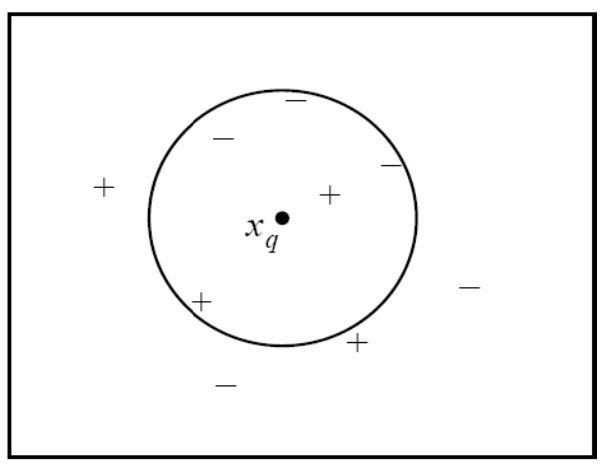
\includegraphics[width=0.34\linewidth,height=0.42\textheight,keepaspectratio]{images/05-knn_1nn-vs-5nn.png}
\caption{1-NN returns ``+'' for \(x_q\), 5-NN returns ``−'': increasing
\(k\) ``smooths'' the decision, useful with noisy data.}
\end{figure}

\begin{figure}[htbp]
\centering
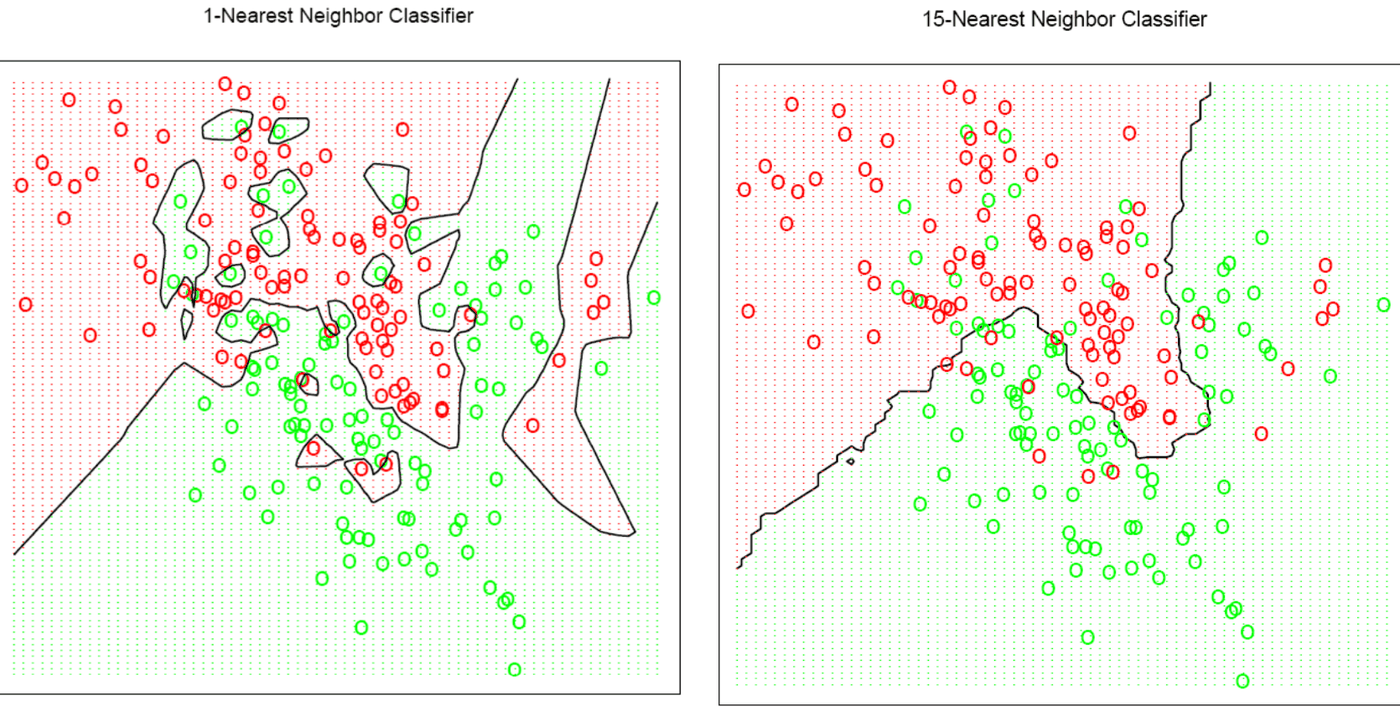
\includegraphics[width=0.89\linewidth,height=0.42\textheight,keepaspectratio]{images/05-knn_1nn-15nn.png}
\caption{Decision boundaries of 1-NN (left) and 15-NN (right) on the
same problem.}
\end{figure}

With \(k = 15\) the model is still very flexible, but makes some errors
on the training set; the boundary is still irregular but less so, and
it \textbf{adapts to the local densities} of the classes.

K-NN implicitly uses the \textbf{Voronoi diagram}: each cell contains
all points closer to a certain pattern than to any other, and the edges
of the cells are the points equidistant from two patterns. 1-NN assigns
to each cell the label of its pattern.

\begin{figure}[htbp]
\centering
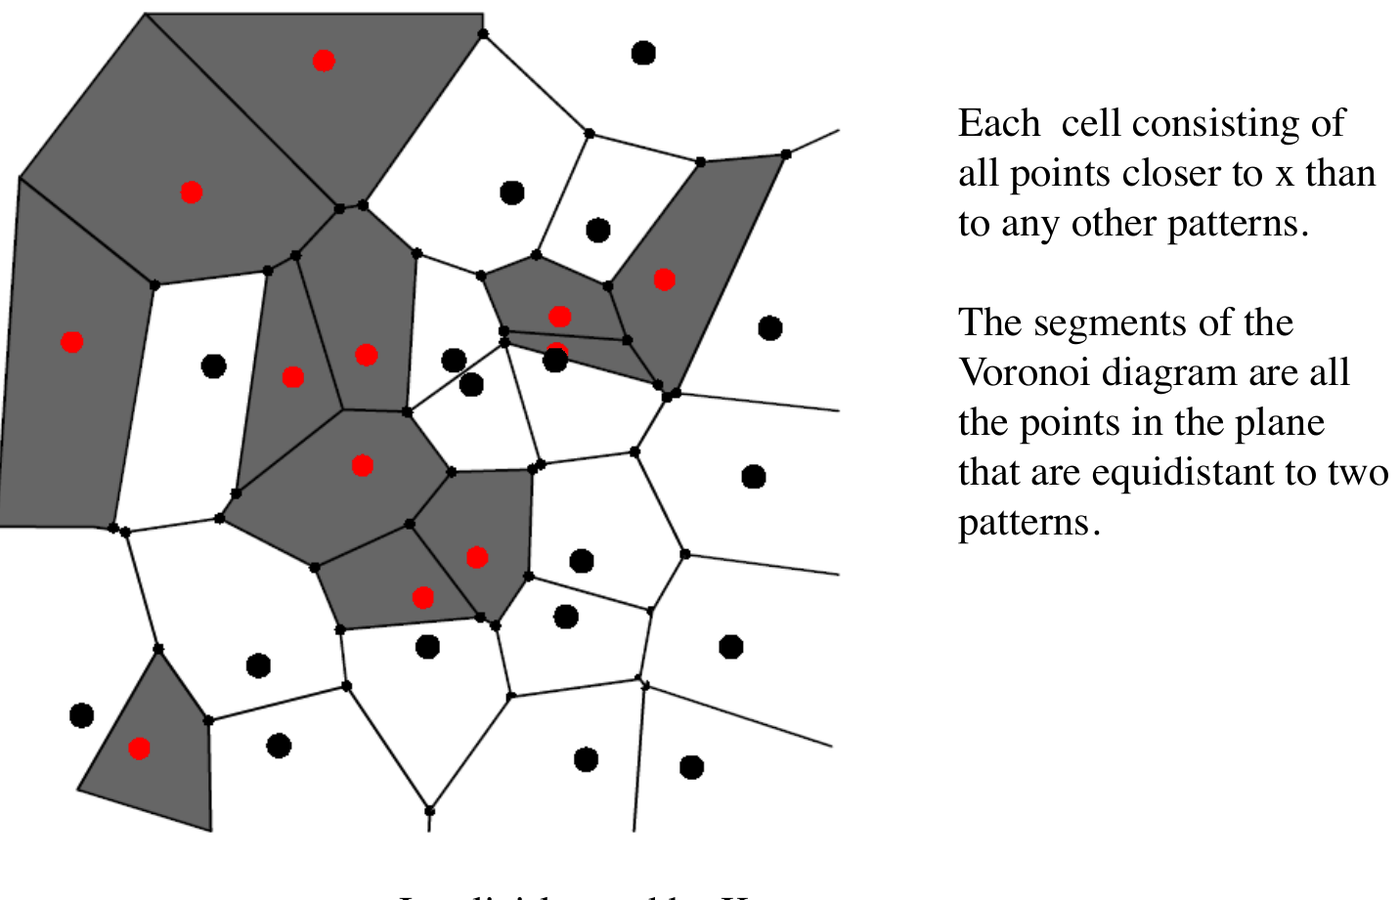
\includegraphics[width=0.69\linewidth,height=0.42\textheight,keepaspectratio]{images/05-knn_voronoi.png}
\caption{Voronoi diagram: the 1-NN boundary follows the edges of the
cells between points of different classes.}
\end{figure}

\subsection{\texorpdfstring{Behaviour as
\(k\) varies}{Behaviour as k varies}}\label{il-comportamento-al-variare-di-k}

In K-NN too we find the \textbf{trade-off between underfitting and
overfitting}, governed by the value of \(k\). The test error has the
classic \textbf{U} shape moving between two extremes:

\begin{itemize}
\tightlist
\item
  \(k = 1\): the \textbf{extremely flexible} case (zero training
  error, jagged boundary, risk of overfitting);
\item
  \(k = l\) (all data): a \textbf{very rigid} model, which answers
  with \textbf{a single average for all data} (for classification, the
  most frequent class in the training set), whatever the input.
\end{itemize}

\begin{figure}[htbp]
\centering
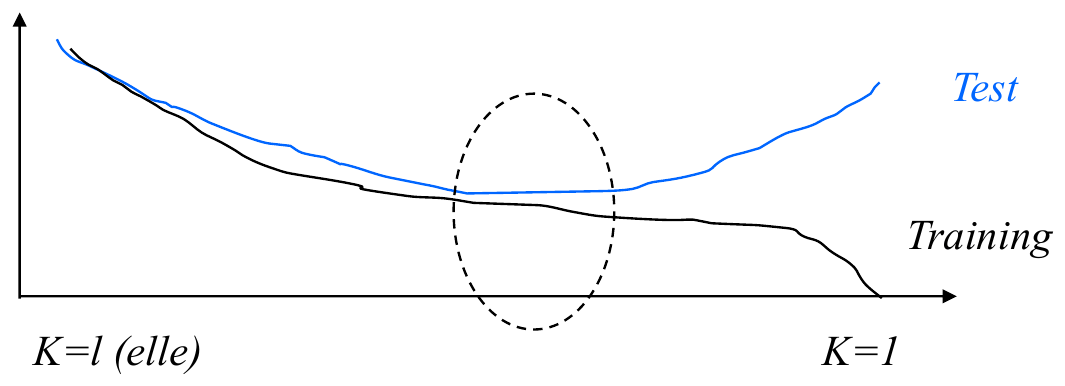
\includegraphics[width=0.63\linewidth,height=0.42\textheight,keepaspectratio]{images/05-knn_u-shape.png}
\caption{K-NN behaviour: from \(k = l\) (rigid) to \(k = 1\) (flexible)
the training error always decreases, the test error is U-shaped.}
\end{figure}

Where have we seen this before? It is the same trend as in
\textbf{polynomial fitting} as the degree \(M\) grows and in the plot
of the SLT \textbf{VC-bound}
(\href{04\%20-\%20Generalizzazione\%20e\%20validazione\%20(introduzione)}{04
- Generalisation and validation (introduction)}): here it is \(k\)
(read from right to left, i.e.\ \(l/k\)) that acts as complexity
control. Intermediate values of \(k\) give the best trade-off.

\subsection{Variants}\label{varianti}

\textbf{Multi-class}: the most frequent class among the \(k\)
neighbours is returned: \[
h(\mathbf{x}) = \arg\max_v \sum_{\mathbf{x}_i \in N_k(\mathbf{x})} \mathbb{1}_{v, y_i}, \qquad \mathbb{1}_{v, y_i} = \begin{cases} 1 & \text{if } v = y_i \\ 0 & \text{otherwise.} \end{cases}
\]

\textbf{Distance-weighted}: closer neighbours count more: \[
h(\mathbf{x}) = \arg\max_v \sum_{\mathbf{x}_i \in N_k(\mathbf{x})} \frac{\mathbb{1}_{v, y_i}}{d(\mathbf{x}, \mathbf{x}_i)^2},
\] and if \(d = 0\) for some \(\mathbf{x}_i\), \(y_i\) is returned
directly.

\subsection{An extreme of ML}\label{un-estremo-del-ml}

K-NN does not build a global hypothesis valid for all instances:
\textbf{there is no model to train}, but the examples must be stored.
It makes \textbf{local} estimates (with locally constant functions)
instead of a global linear approximation. It is a \emph{lazy} method,
memory-based, instance-based, distance-based.

\subsection{K-NN versus linear
model}\label{k-nn-contro-modello-lineare}

{\def\LTcaptype{none} % do not increment counter
\begin{longtable}[]{@{}
  >{\raggedright\arraybackslash}p{(\linewidth - 4\tabcolsep) * \real{0.3333}}
  >{\raggedright\arraybackslash}p{(\linewidth - 4\tabcolsep) * \real{0.3333}}
  >{\raggedright\arraybackslash}p{(\linewidth - 4\tabcolsep) * \real{0.3333}}@{}}
\toprule\noalign{}
\begin{minipage}[b]{\linewidth}\raggedright
\end{minipage} & \begin{minipage}[b]{\linewidth}\raggedright
Linear
\end{minipage} & \begin{minipage}[b]{\linewidth}\raggedright
K-NN
\end{minipage} \\
\midrule\noalign{}
\endhead
\bottomrule\noalign{}
\endlastfoot
Flexibility & rigid (\textbf{low variance}) & flexible (\textbf{high
variance}) \\
Timing & eager & lazy \\
Type & parametric & instance-based \\
Parameters & \(n+1\) (3 in the example) & about \(l/k\) ``effective
parameters'' \\
\end{longtable}
}

With small \(k\) a few points are enough to change the boundary:
flexibility comes at a price. One might think that K-NN has a single
parameter (\(k\)), but realistically it has about \textbf{\(l/k\)
effective parameters} (Hastie-Tibshirani-Friedman): it is as if it
divided the space into \(l/k\) regions, each with its own ``mean''.

\begin{figure}[htbp]
\centering
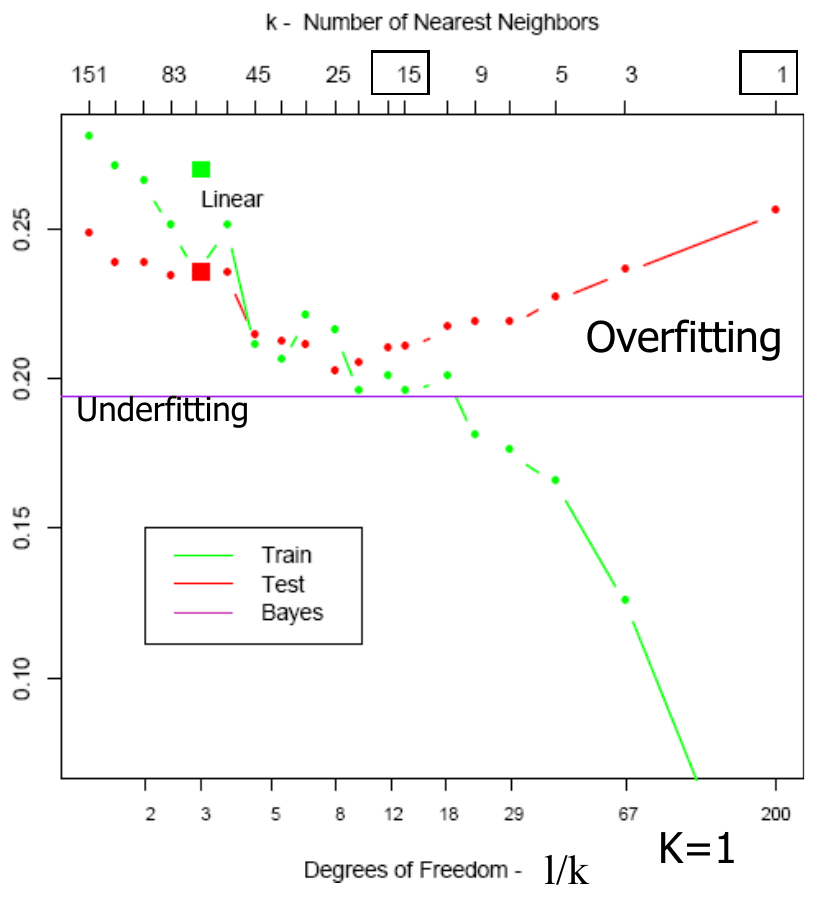
\includegraphics[width=0.54\linewidth,height=0.42\textheight,keepaspectratio]{images/05-knn_errori-k.png}
\caption{K-NN error curves as \(k\) varies (training of 200 points, test
of 10000). The squares are the linear model, the purple line the
optimal Bayes error.}
\end{figure}

Moving from large \(k\) to \(k = 1\) (i.e.\ increasing \(l/k\)) we go
from \textbf{underfitting} to \textbf{overfitting}: the training error
drops to zero, the test error has a minimum for intermediate values.
It is again the SLT bound plot, with \(k\) in the role of complexity
control: more flexibility makes it possible to find the best result,
\textbf{if} complexity is controlled.

\subsection{The Bayes optimal
classifier}\label{il-classificatore-ottimo-di-bayes}

\begin{boxdefinition}{Bayes classifier and Bayes error}

If the density \(P(\mathbf{x}, y)\) is known, the optimal choice is to
assign the most probable class: \[
h(\mathbf{x}) = \arg\max_v P(v \mid \mathbf{x}), \qquad v \in \{C_1, \dots, C_K\}.
\] Its error rate, called the \textbf{Bayes rate}, is the
\textbf{minimum achievable error} given the data distribution
(assuming the generating density is known).

\end{boxdefinition}

K-NN directly approximates this solution: the majority vote in a
neighbourhood is exactly an estimate of
\(\arg\max_v P(v \mid \mathbf{x})\), with two relaxations: the
conditional probability \textbf{at a point} becomes the conditional
probability \textbf{in a neighbourhood} of the point (local
approximation), and probabilities are estimated with the
\textbf{proportions} in the training sample.

\begin{figure}[htbp]
\centering
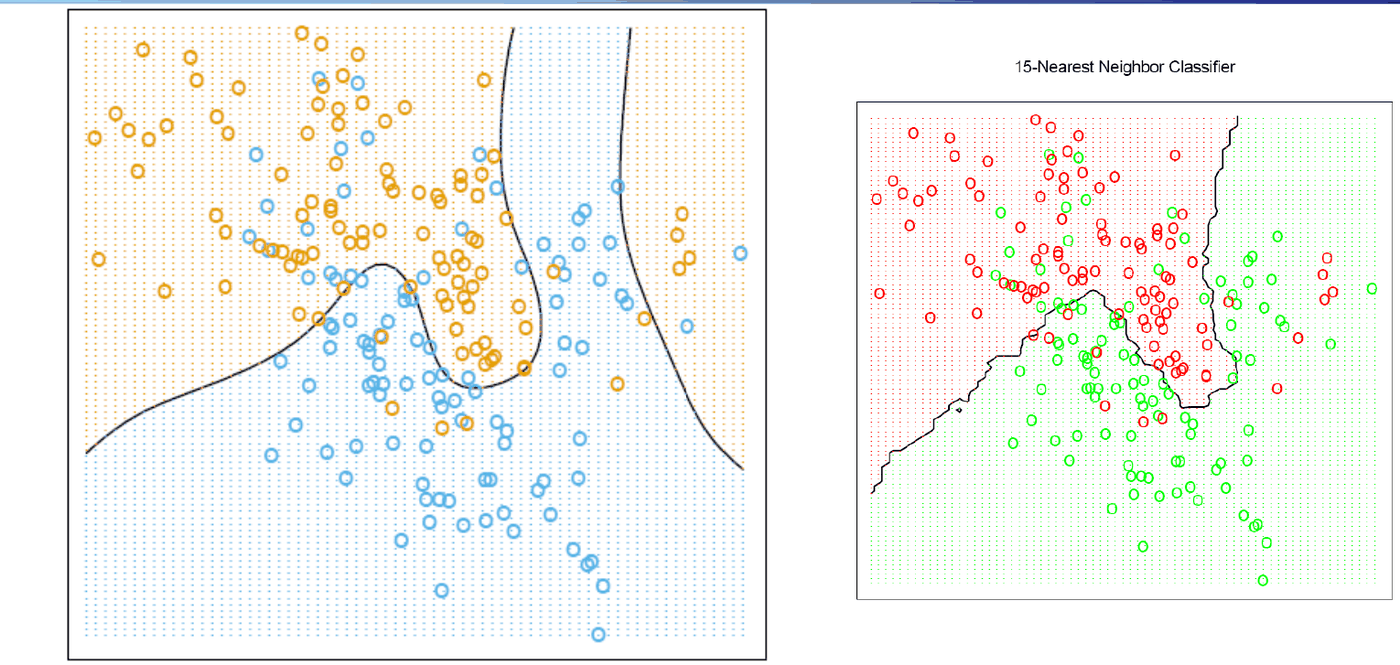
\includegraphics[width=0.80\linewidth,height=0.42\textheight,keepaspectratio]{images/05-knn_bayes.png}
\caption{Optimal Bayes boundary (left) and 15-NN boundary (right): the
15-NN is very close to the optimum, consistently with the minimum of
the test error in the previous figure.}
\end{figure}

\subsection{Inductive bias of K-NN}\label{bias-induttivo-del-k-nn}

\begin{enumerate}
\def\labelenumi{\arabic{enumi}.}
\tightlist
\item
  \textbf{The assumed distance} establishes which examples are
  similar: it is assumed that the classification of a point is similar
  to that of its neighbours \textbf{according to the chosen metric}.
  Metrics other than the Euclidean one can be used; symbolic data
  require ad hoc metrics (e.g.\ the \textbf{Hamming distance} between
  strings of the same length: the number of positions in which they
  differ).
\item
  \textbf{Locality}: local approximation, with an assumption of local
  \emph{smoothness} (to be compared later with the bias of deep
  learning).
\end{enumerate}

The bias related to the metric is often underestimated in books, but
it is crucial.

\subsection{Limits of K-NN}\label{limiti-del-k-nn}

\subsubsection{Variable scale and
metric}\label{scala-delle-variabili-e-metrica}

The choice of scale depends on domain knowledge. If the variables must
contribute equally, one must pay attention to differences in range:
\textbf{rescaling the data} (e.g.\ zero mean and unit variance) is
equivalent to \textbf{changing the metric}. Scaling can completely
change which is the nearest neighbour: K-NN is fragile even with
respect to elementary pre-processing.

\begin{figure}[htbp]
\centering
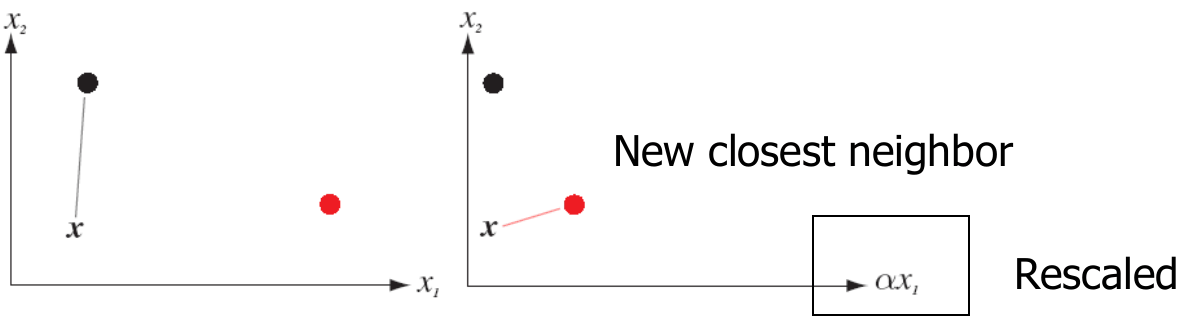
\includegraphics[width=0.71\linewidth,height=0.42\textheight,keepaspectratio]{images/05-knn_scala.png}
\caption{Rescaling a variable changes the nearest neighbour.}
\end{figure}

\subsubsection{Computational cost}\label{costo-computazionale}

K-NN builds the local approximation \textbf{for each new example} to be
predicted: the computational cost is \textbf{shifted to the prediction
phase}. For each input the distances from all stored vectors are
computed (time proportional to the number of patterns), although there
are ad hoc proximity search algorithms, such as pattern indexing or
\textbf{approximate nearest neighbor search} techniques, which give up
always finding the exact neighbour in exchange for a much faster
search. The \textbf{space} cost is also high (all the training data).

\subsubsection{Interpretability}\label{interpretabilituxe0}

K-NN models offer little interpretation, subjective and dependent on
the metric.

\subsubsection{The curse of
dimensionality}\label{la-maledizione-della-dimensionalituxe0}

K-NN works well if a significant set of data close to each
\(\mathbf{x}\) can be found, i.e.\ with \textbf{dense sampling}. When
there are many input variables (high dimension \(n\)) it often fails
because of the \textbf{curse of dimensionality}, which has many
manifestations. Three in particular directly affect generalisation.

\textbf{1. In high dimension it is hard to find close points.} It
becomes difficult to collect \(k\) observations ``close'' (i.e.\
similar) to a query point: neighbourhoods tend to be spatially large
and estimates are no longer local; reducing the size of the
neighbourhood means reducing \(k\), and the variance of the estimate
increases (overfitting).

Consider data uniformly distributed in the unit cube and a sub-cube
that must contain a fraction \(r\) of the data. Its side must be
\(r^{1/n}\) (since volume \(=\) side\(^n\)).

\begin{figure}[htbp]
\centering
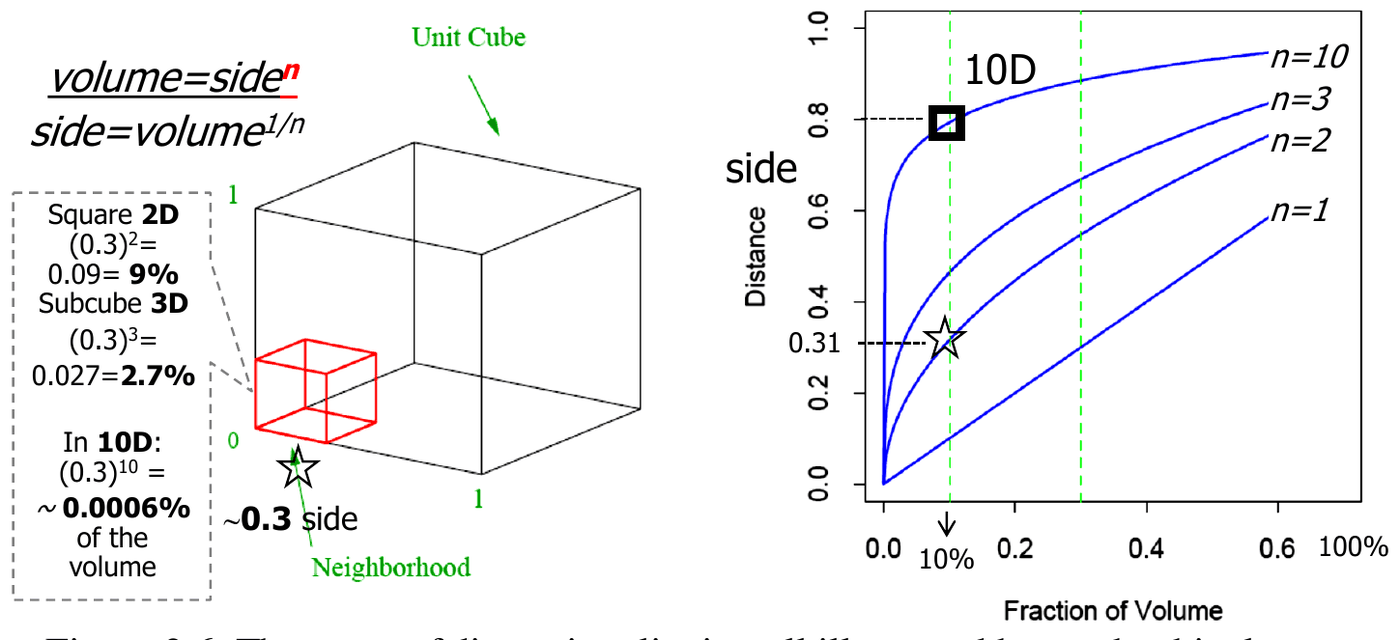
\includegraphics[width=0.86\linewidth,height=0.42\textheight,keepaspectratio]{images/05-knn_curse.png}
\caption{Curse of dimensionality: side of the sub-cube needed to capture
a fraction \(r\) of the volume, as the dimension \(n\) varies.}
\end{figure}

\begin{itemize}
\tightlist
\item
  To capture 10\% of the data: in 2D a side of
  \(0.1^{1/2} \approx 0.32\) is enough (30\% of the range of each
  variable); in 10D \(0.1^{1/10} \approx 0.8\) is needed, i.e.\
  \textbf{80\% of the range} of each coordinate! Even for 1\% of the
  volume in 10D, 63\% of the range is needed. The neighbourhood is no
  longer ``local'' and the neighbours are no longer similar.
\item
  Conversely, fixing the side at 0.3: in 1D we capture 30\% of the
  data, in 2D 9\%, in 3D 2.7\%, in 10D about \textbf{0.0006\%}. That
  side may not be enough to find \(k\) data points, unless a small
  \(k\) is used (and thus risking overfitting).
\end{itemize}

\textbf{2. Low sampling density.} The sampling density is proportional
to \(l^{1/n}\). If 100 points are enough to estimate a function in
\(\mathbb{R}^1\), to obtain similar accuracy in \(\mathbb{R}^{10}\)
\(100^{10} = 10^{20}\) are needed.

\textbf{3. Irrelevant features} (\emph{curse of noisy}). If the target
depends only on a few of the many features (e.g.\ 2 out of 20), the
similarity between patterns can be dominated by the large number of
irrelevant features, and the ``neighbour'' found is not really
similar. The problem grows with dimensionality. Remedies:
\textbf{weighting the features} according to their relevance
(stretching the axes along some dimensions; the weights can be searched
with an expensive model selection or other methods) or performing
\textbf{feature selection} (eliminating variables, reducing the input
dimension).

\subsection{K-NN design
choices}\label{scelte-di-progetto-del-k-nn}

\begin{itemize}
\tightlist
\item
  The \textbf{metric} \(d\) (Euclidean, Hamming, Manhattan, feature
  weights\ldots): it is often the key to the success of an
  application.
\item
  The value of \textbf{\(k\)}, which controls underfitting and
  overfitting.
\item
  It is often necessary to select a \textbf{subset of the data} (a set
  of prototypes, for example via clustering) and a \textbf{subset of
  the features}.
\end{itemize}

Extensions to other local models: \emph{kernel smoothers}, local linear
regression, prototype methods, \emph{case-based reasoning}.

\begin{boxabstract}{General lessons from K-NN}

\begin{itemize}
\tightlist
\item
  Too low a variance is poor (rigid linear models), too high a
  variance is dangerous (K-NN).
\item
  \textbf{Smoothing}: in K-NN it is obtained by increasing \(k\).
\item
  \textbf{Curse of dimensionality}: the volume of the space grows so
  fast that the data become sparse.
\item
  The error curves as \(k\) varies are another instance of the SLT
  bound plot.
\item
  The inductive bias of K-NN is related to the metric.
\end{itemize}

\end{boxabstract}

\subsection{What next?}\label{e-adesso}

K-NN does not build a real ``learned model'': it does not extract
regularities or synthesise knowledge, and it does not satisfy the goal
of learning (being able to ``forget'' the examples after building the
model). In the next lectures we look for models that are
\textbf{compact} like the LTU (all knowledge in a few parameters) but
\textbf{flexible} like K-NN, with adequate support for complexity
control: \textbf{neural networks}.

The professor suggests looking at the slides of the following lectures
in advance, and in particular at the \textbf{proof of the Perceptron
convergence theorem}
(\href{06\%20-\%20Reti\%20neurali\%20(parte\%201)\%20-\%20dal\%20neurone\%20al\%20MLP}{06
- Neural networks (part 1) - from the neuron to the MLP}).

\begin{boxquestion}{Possible exam questions}

\begin{itemize}
\tightlist
\item
  Formulate the learning problem for a linear model with LMS, for
  regression and classification.
\item
  Derive the gradient of the squared error and the normal equations.
\item
  Describe the gradient descent algorithm; difference between batch
  and on-line; role of \(\eta\).
\item
  Explain the delta rule as an error-correction rule.
\item
  Why is the squared error on \(\mathbf{w}^T\mathbf{x}\) used for
  classification instead of the 0/1 loss?
\item
  What is linear separability? Why is XOR not linearly separable?
\item
  What is linear basis expansion? Pros and cons.
\item
  Write the Tikhonov loss, the direct solution and the weight decay
  rule; role of \(\lambda\).
\item
  Difference between L1 and L2 regularisation.
\item
  Describe K-NN; compare it with the linear model; what is the Bayes
  classifier?
\item
  Explain the curse of dimensionality.
\end{itemize}

\end{boxquestion}
